\chapter{Validation of the Theoretical Model and the Numerical Simulations}
\label{ch:validation}

The validation is organised as three separate comparisons:
\begin{enumerate}
\item the present CFD against what Delon \emph{et al.} published (\cref{sec:val_published});
\item the present CFD against the three levels of theory (\cref{sec:val_pressure,sec:val_shear,sec:val_transverse,sec:val_velocity,sec:val_cross,sec:val_offset,sec:val_scaling});
\item a physical interpretation of the flow field (\cref{sec:val_physics}).
\end{enumerate}
No single matching variable is taken to validate the model as a whole. Each conclusion is classified separately in \cref{tab:validation_matrix}.

\section{Comparison with the published results}
\label{sec:val_published}

The reference paper gives its results as plots and as ranges in the text and tables. It provides no tabulated curves, and the published curves were not digitised for this report, so a point-by-point RMSE against the paper cannot be computed. The comparison therefore uses the values the paper states explicitly (\cref{tab:published_compare}).

\begin{table}[htbp]
\centering
\caption{Published values \tagP\ \citep{Delon2020} compared with the present CFD \tagC\ and Eq.~2 evaluated for the present geometry \tagT. Shear in \si{\dyncm}. ``Upper/lower'' are the extreme values along the axis of the cell-culture section. $\tau_{\mathrm{cell}}=3\taw$ follows the paper.}
\label{tab:published_compare}
\small
\resizebox{\linewidth}{!}{%
\begin{tabular}{@{}llccc@{}}
\toprule
Quantity & $Q$ & Published \tagP & Present CFD \tagC & Eq.~2, $L=\SI{50}{mm}$ \tagT\\
\midrule
$\taw$ upper (inlet) & 0.22 & $\sim$0.01 & 0.0102 & 0.0098\\
$\taw$ lower (outlet end) & 0.22 & $\sim$0.001 & 0.0014 (min.\ at $x=\SI{44.0}{mm}$) & 0.0010 at \SI{45}{mm}\\
$\taw$ upper (inlet) & 1 & 0.0447 & 0.0464 & 0.0447\\
$\taw$ lower (outlet end) & 1 & 0.0059 & 0.0063 (min.\ at $x=\SI{44.0}{mm}$) & 0.0045 at \SI{45}{mm}\\
$\tau_{\mathrm{cell}}$ range, CFD & 0.22 & $\sim$0.03 -- 0.003 & 0.030 -- 0.0042 & --\\
$\tau_{\mathrm{cell}}$ range, CFD & 1 & $\sim$0.134 -- 0.017 & 0.139 -- 0.019 & --\\
$\tau_{\mathrm{cell}}$ range, equation & 1 & 0.135 -- 0.008 & -- & 0.134 -- 0.013\\
Uniform-zone width independent of $Q$ & all & yes (stated) & yes, $<\SI{0.002}{mm}$ & yes (Stokes flow)\\
\bottomrule
\end{tabular}}
\end{table}

\paragraph{Shear magnitude and range.} The present CFD reproduces the published shear range at both flow rates. At the inlet it is within \SI{2}{\percent} (0.22) and \SI{4}{\percent} (1) of the published values. At the downstream end both studies find a minimum that lies \emph{above} the end value of Eq.~2 (0.0063 here against 0.0059 published, both above 0.0045). This agrees with T3: the outlet corner raises the shear near $x_t$ (\cref{sec:th_T3}). The published equation range for \SI{1}{\uLmin} (0.135--\SI{0.008}{\dyncm}) is consistent with evaluating Eq.~2 with $L=\SI{5.3}{cm}$ up to $x\approx\SI{5.0}{cm}$, since $0.134\times(1-5.0/5.3)\approx0.0076$. This is our inference; the paper does not state it. It explains why the published equation and CFD lower bounds differ by a factor of two, while the present comparison at matched positions does not.

\paragraph{Uniform-shear zone.} \Cref{fig:published_d} compares the published imaging zone with the present one. At S3 and S4 the present half-width at $\pm\SI{5}{\percent}$ (0.834 and \SI{1.518}{mm}) agrees with the published $D_{\max}$ (0.82 and \SI{1.5}{mm}) to within \SI{2}{\percent}. At S1 and S2 the present zone is 15--\SI{17}{\percent} wider; the published values are close to (S1) or below (S2) the present half-widths at the strict $\pm\SI{2}{\percent}$ tolerance. The published wall layers $D_{\mathrm{wall}}$ (0.16--\SI{0.24}{mm}) are of the same order as the present ones (0.15--\SI{0.17}{mm}) and the theory (\SI{0.129}{mm}). At S5 the two studies disagree strongly (3.84 against \SI{1.02}{mm}). The present value is confirmed by T3 (\SI{1.05}{mm}). The published $D_{\mathrm{wall}}+D_{\max}=\SI{4.17}{mm}$ at S5 does not equal the present half-width of \SI{5}{mm}, which suggests a different planform near the corner (e.g.\ $L=\SI{53}{mm}$) or a different criterion. Since the paper's criterion for ``constant'' shear is not stated, these comparisons are semi-quantitative.

\begin{figure}[htbp]
\centering
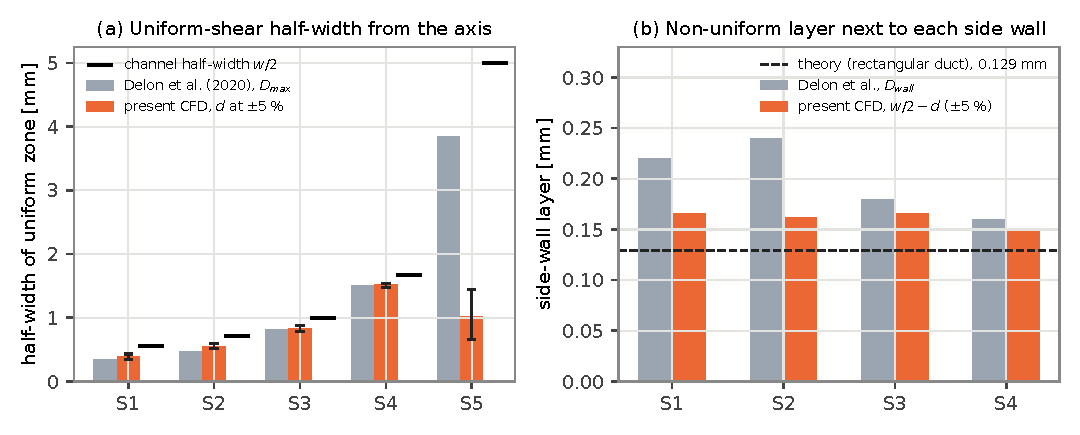
\includegraphics[width=\linewidth]{published_vs_present_uniform_zone.pdf}
\caption{Imaging zone of Delon \emph{et al.} (Table~2 of \citep{Delon2020}) compared with the present CFD at \SI{1}{\uLmin}. (a) Half-width of the uniform-shear band; error bars span the present results at $\pm2$ and $\pm\SI{10}{\percent}$ tolerance. (b) Width of the non-uniform layer at each side wall, with the rectangular-duct theory, \cref{eq:th_delta}.}
\label{fig:published_d}
\end{figure}

\paragraph{Assessment.} The published flow behaviour is reproduced \emph{qualitatively and semi-quantitatively}. The present results reproduce the linear shear decrease, the shear range at both flow rates to within a few percent, the raised minimum near the outlet, the imaging zones at S3--S4 and the independence of the flow rate. Exact agreement cannot be expected, for three reasons: the paper's own height and length are inconsistent (\cref{ch:lit}), its curves are available only as plots, and its uniformity criterion is not specified.

\section{Pressure distribution}
\label{sec:val_pressure}

\Cref{fig:contours}a shows the Fluent pressure contours. The pressure falls smoothly from inlet to outlet. Iso-bars are straight across the narrow part, as \cref{eq:th_dpdx_general} assumes, and bend only near the outlet corner, where the flow becomes two-dimensional. The colour-bar maxima scale with $Q$ to within \SI{0.3}{\percent} (1.795--\SI{1.800}{Pa} per \ulmin).

\begin{figure}[htbp]
\centering
\begin{subfigure}[t]{0.49\linewidth}\centering
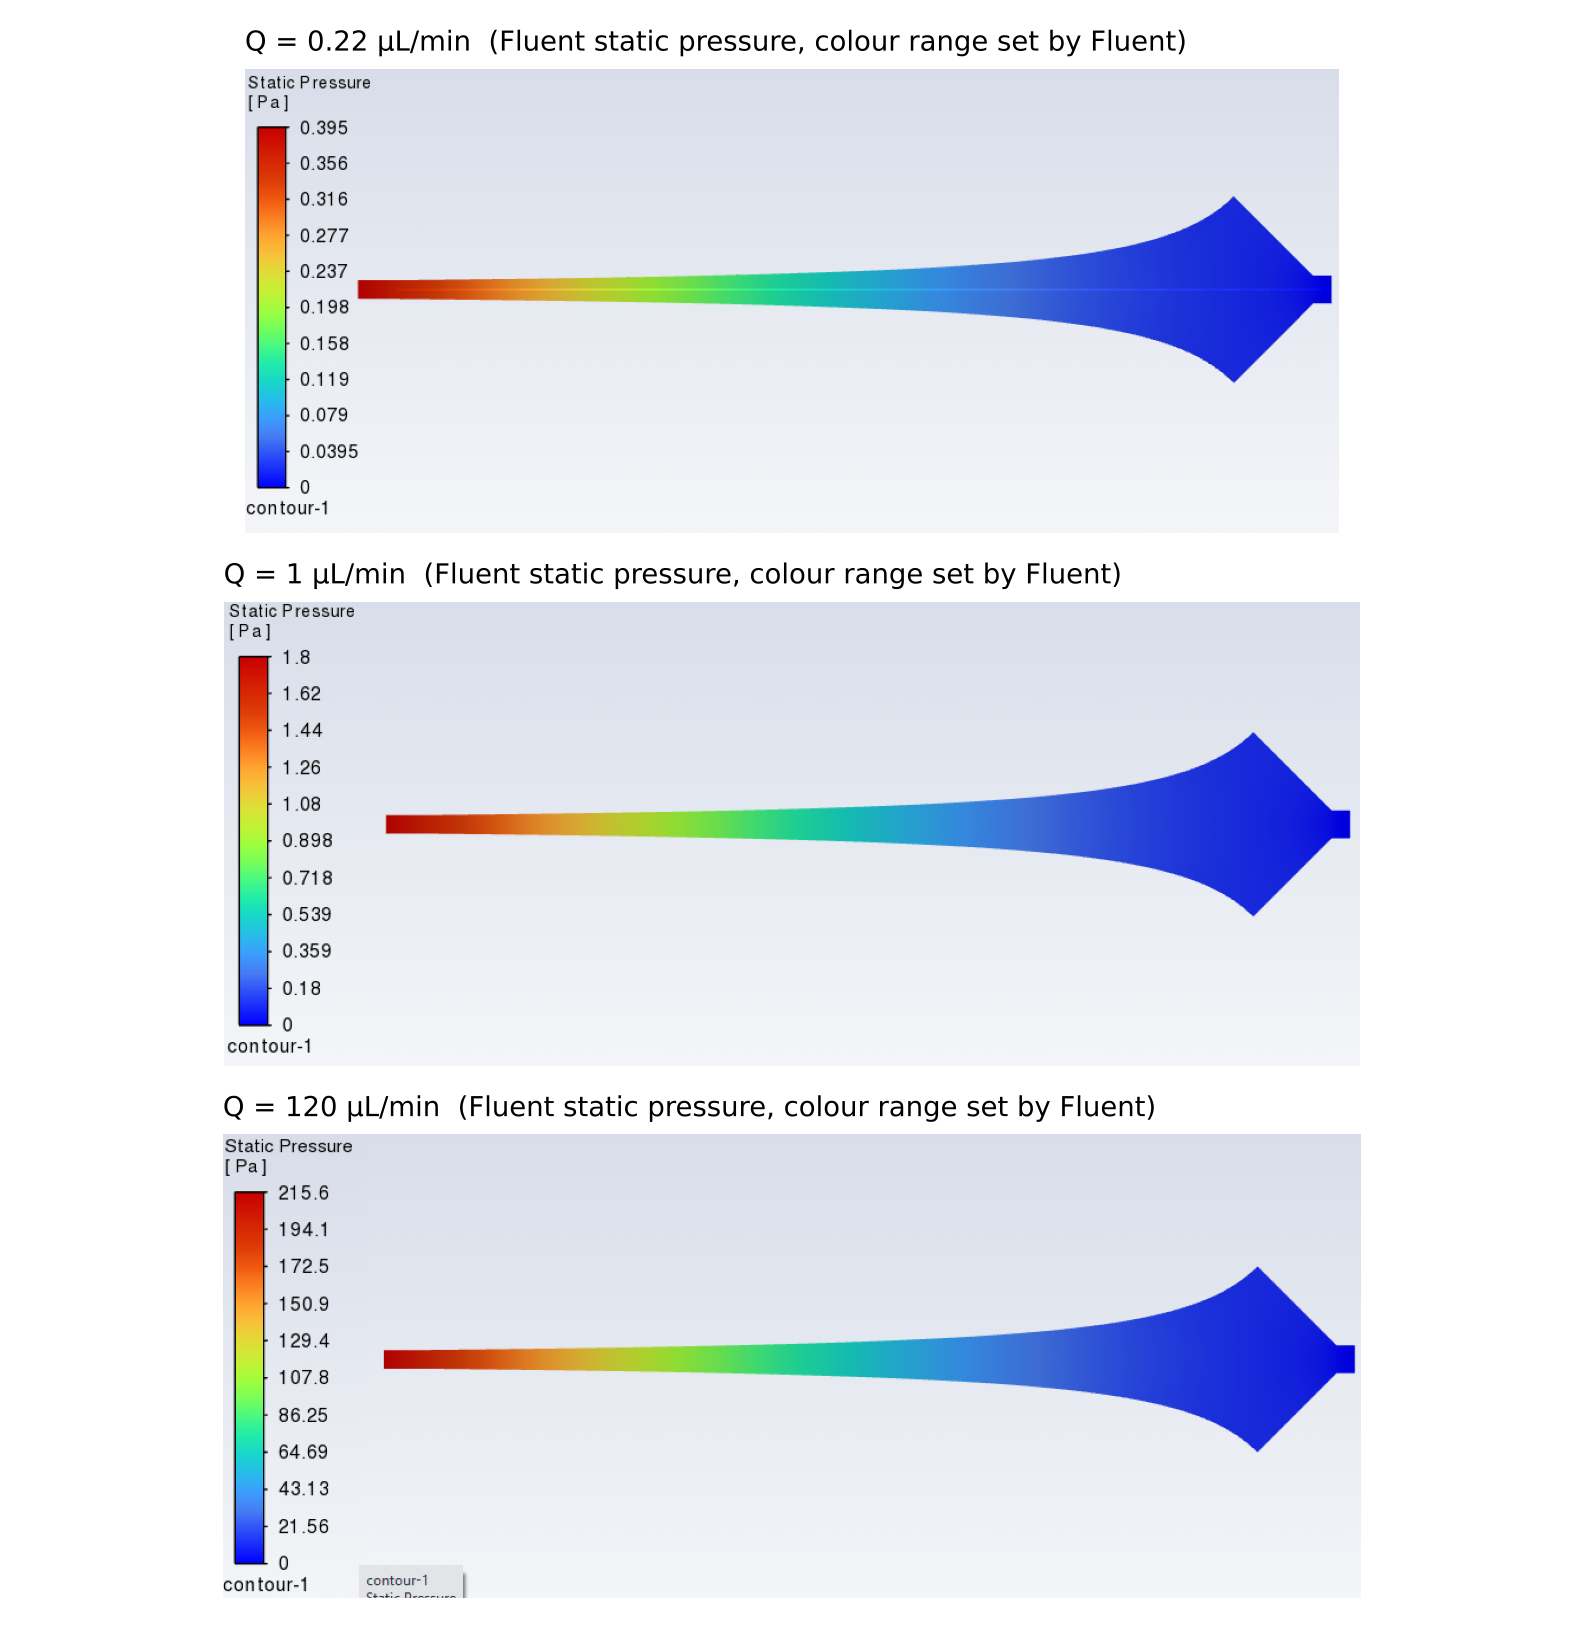
\includegraphics[width=\linewidth]{Fig01_pressure_contours_all_Q.png}
\caption{Static pressure.}
\end{subfigure}\hfill
\begin{subfigure}[t]{0.49\linewidth}\centering
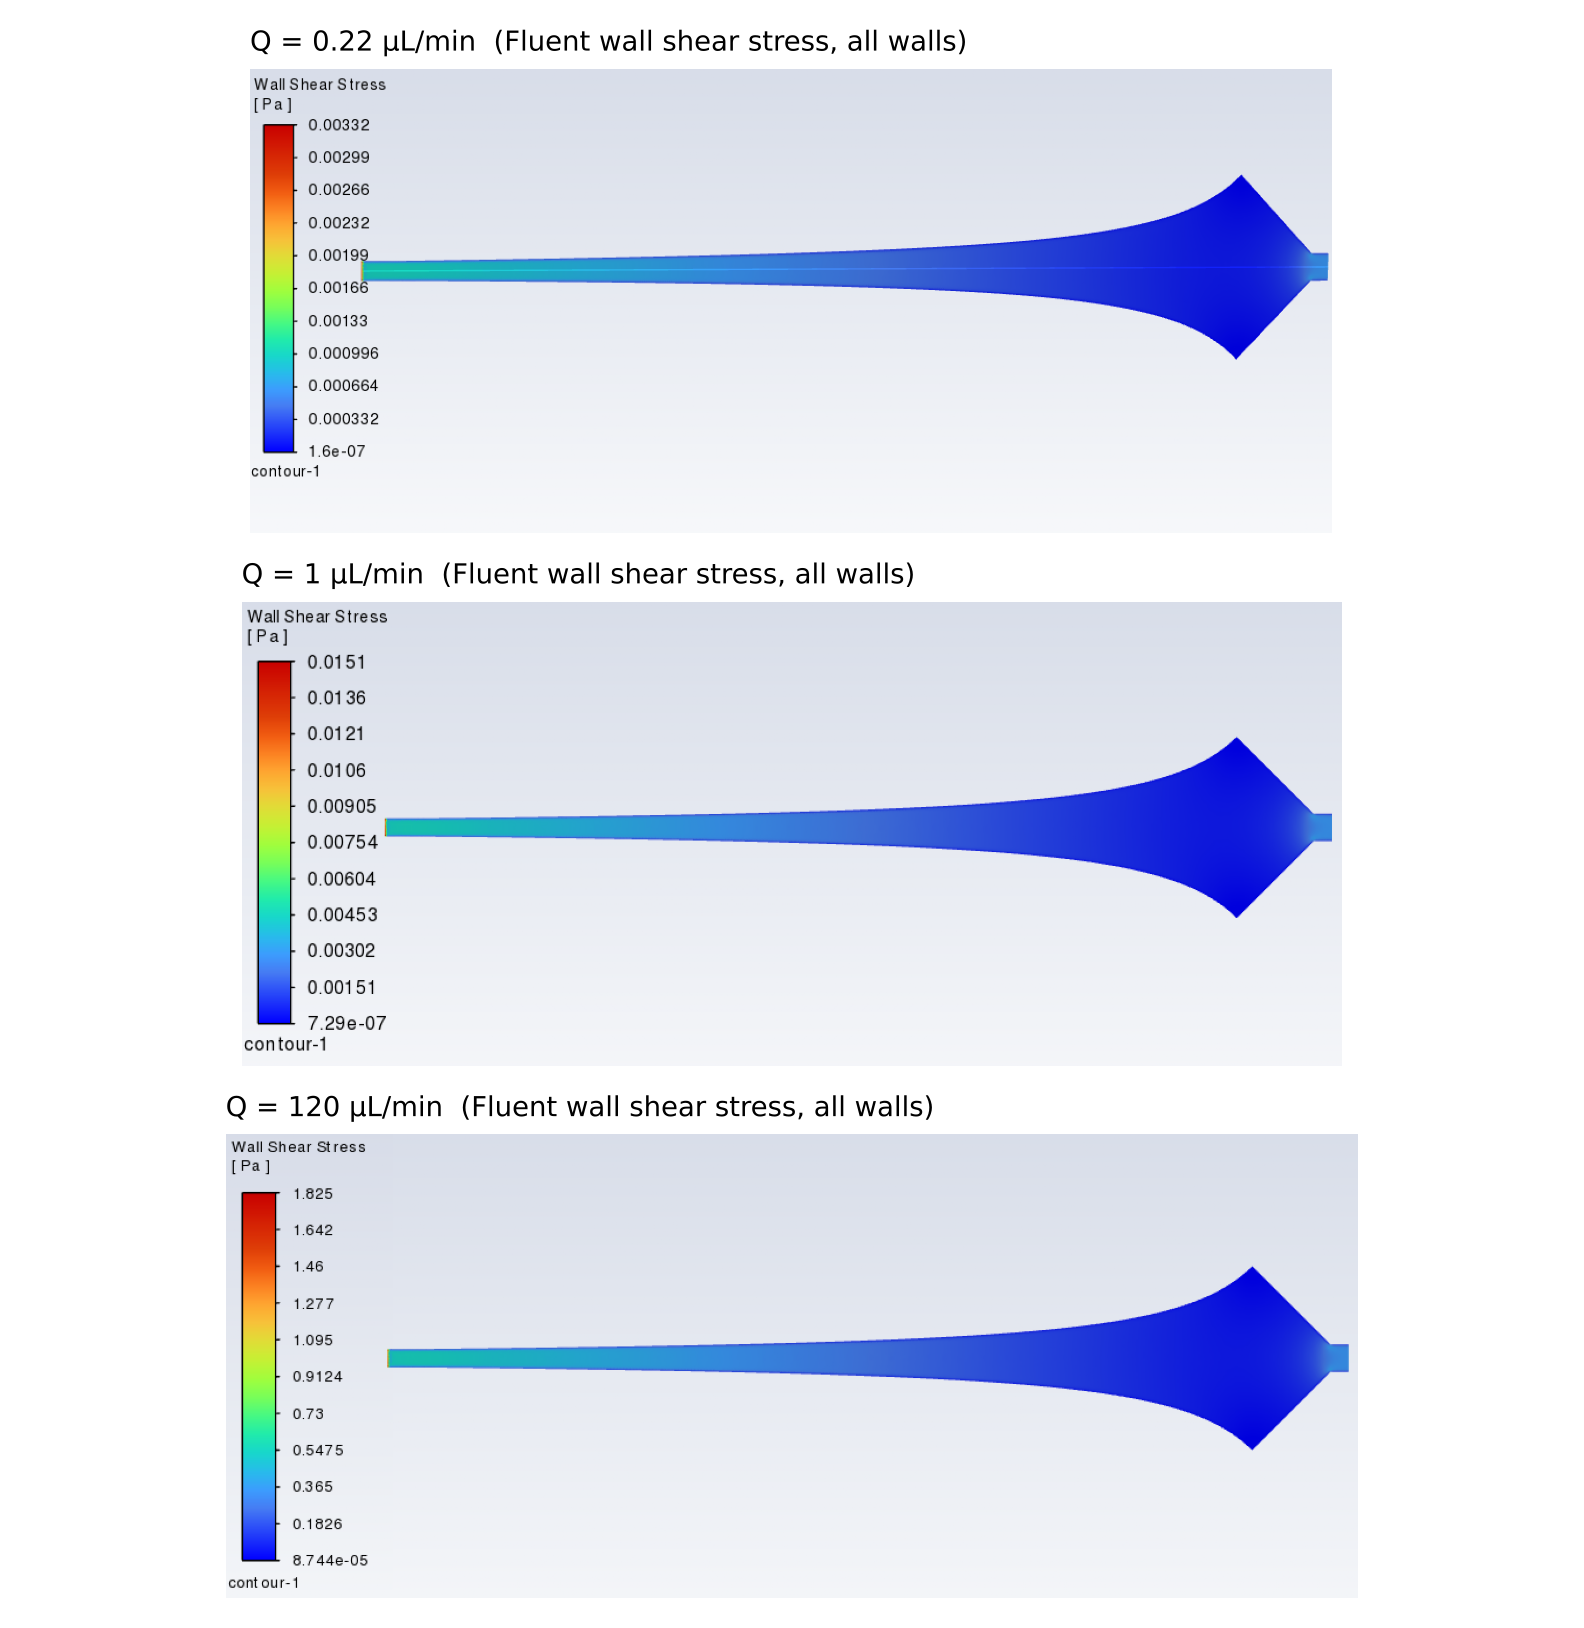
\includegraphics[width=\linewidth]{Fig09_wall_shear_contours_all_Q.png}
\caption{Wall shear stress.}
\end{subfigure}
\caption{Fluent contours at 0.22 (top), 1 (middle) and \SI{120}{\uLmin} (bottom) \tagC. These are raster screenshots with automatic colour ranges. The pressure maxima (0.395, 1.80 and \SI{215.6}{Pa}) include the \SI{2}{mm} lead-in. The wall-shear maxima (\num{3.32e-3}, \num{1.51e-2} and \SI{1.825}{Pa}) occur at the inlet face of the lead-in, where the uniform inlet velocity creates a local peak. This peak dominates the colour scale, so the shear gradient along the cell floor is quantified in the line plots that follow.}
\label{fig:contours}
\end{figure}

\Cref{fig:p_axis} compares the axial pressure at \SI{1}{\uLmin} with the theory. It decreases monotonically: none of the 729 successive differences is positive in any case. The profile flattens along the widening section, because a wider channel needs a smaller gradient for the same flow, and it steepens again where the walls converge to the outlet. T3 reproduces the whole shape, including the outlet region, but lies about \SI{5}{\percent} above the CFD everywhere. Normalised by $Q$, the three cases collapse onto one curve (\cref{fig:p_norm}). The pressure drop from $x=0$ to the outlet is $\Delta p=1.657\,Q$ (Pa, $Q$ in \ulmin) with $R^2=1.000000$ (\cref{fig:dp_Q}). The hydraulic resistance is \SI{9.94e10}{Pa.s/m^3} at all three flow rates, varying by only \SI{0.02}{\percent}.

\begin{figure}[htbp]
\centering
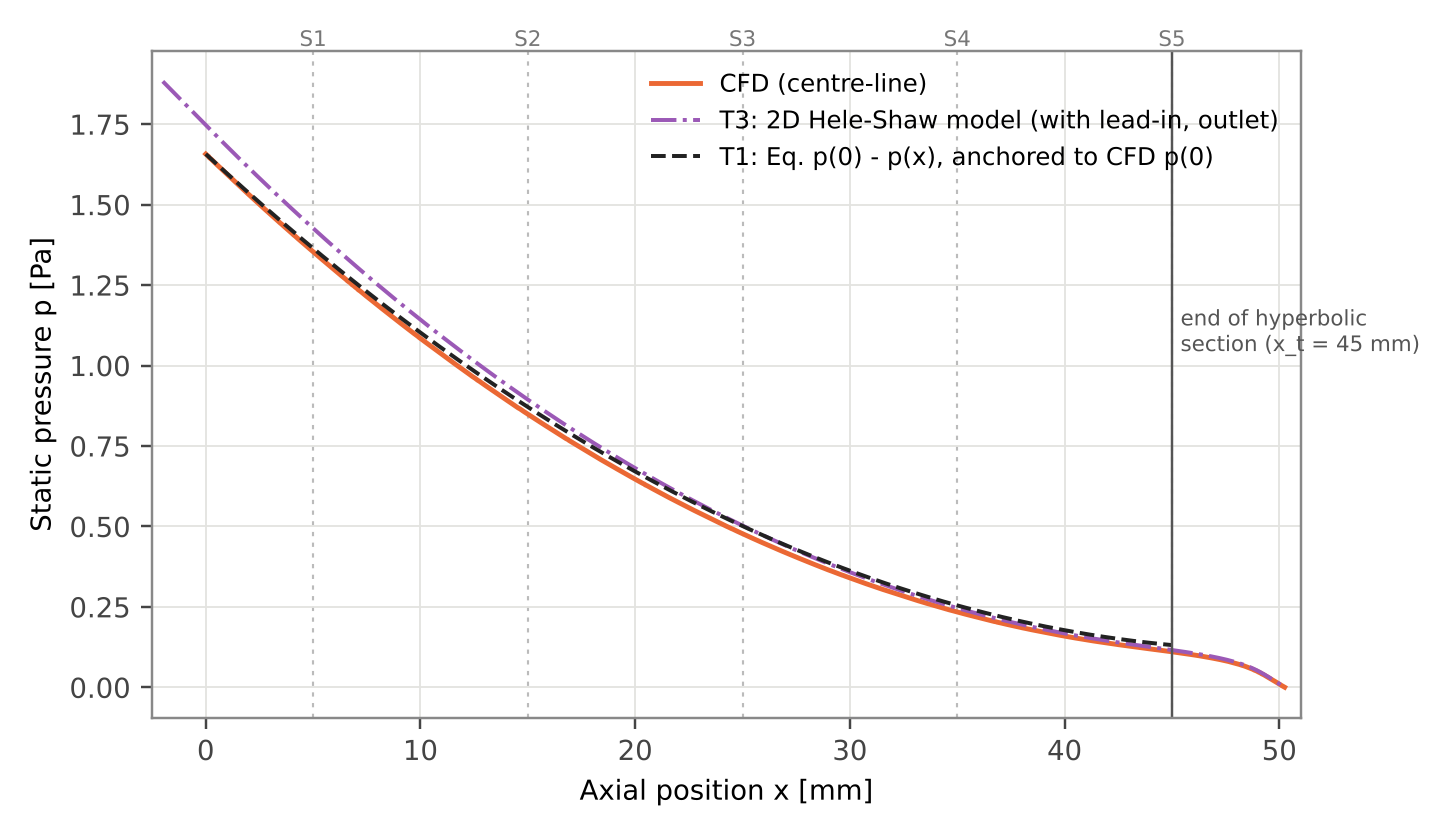
\includegraphics[width=0.85\linewidth]{Fig03_pressure_vs_x_Q1.png}
\caption{Static pressure along the axis at \SI{1}{\uLmin}: CFD \tagC\ against T3 (absolute; includes the lead-in and the outlet transition) and T1, \cref{eq:th_p}, anchored at the CFD value at $x=0$ \tagT. T1 applies only to $0\le x\le\SI{45}{mm}$.}
\label{fig:p_axis}
\end{figure}

\begin{figure}[htbp]
\centering
\begin{subfigure}[t]{0.49\linewidth}\centering
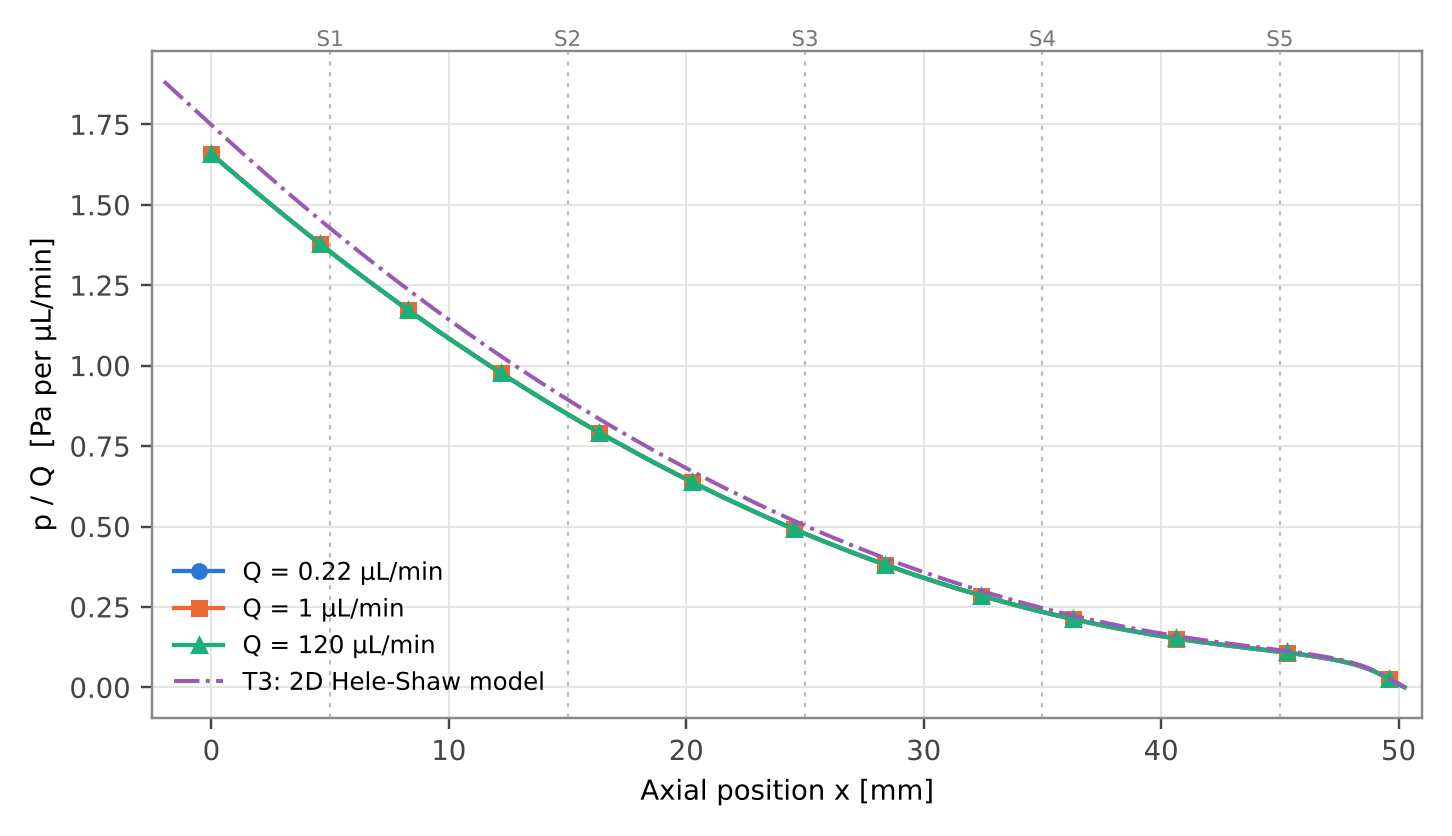
\includegraphics[width=\linewidth]{Fig05_pressure_vs_x_combined_normalised.png}
\caption{Pressure divided by $Q$.}\label{fig:p_norm}
\end{subfigure}\hfill
\begin{subfigure}[t]{0.49\linewidth}\centering
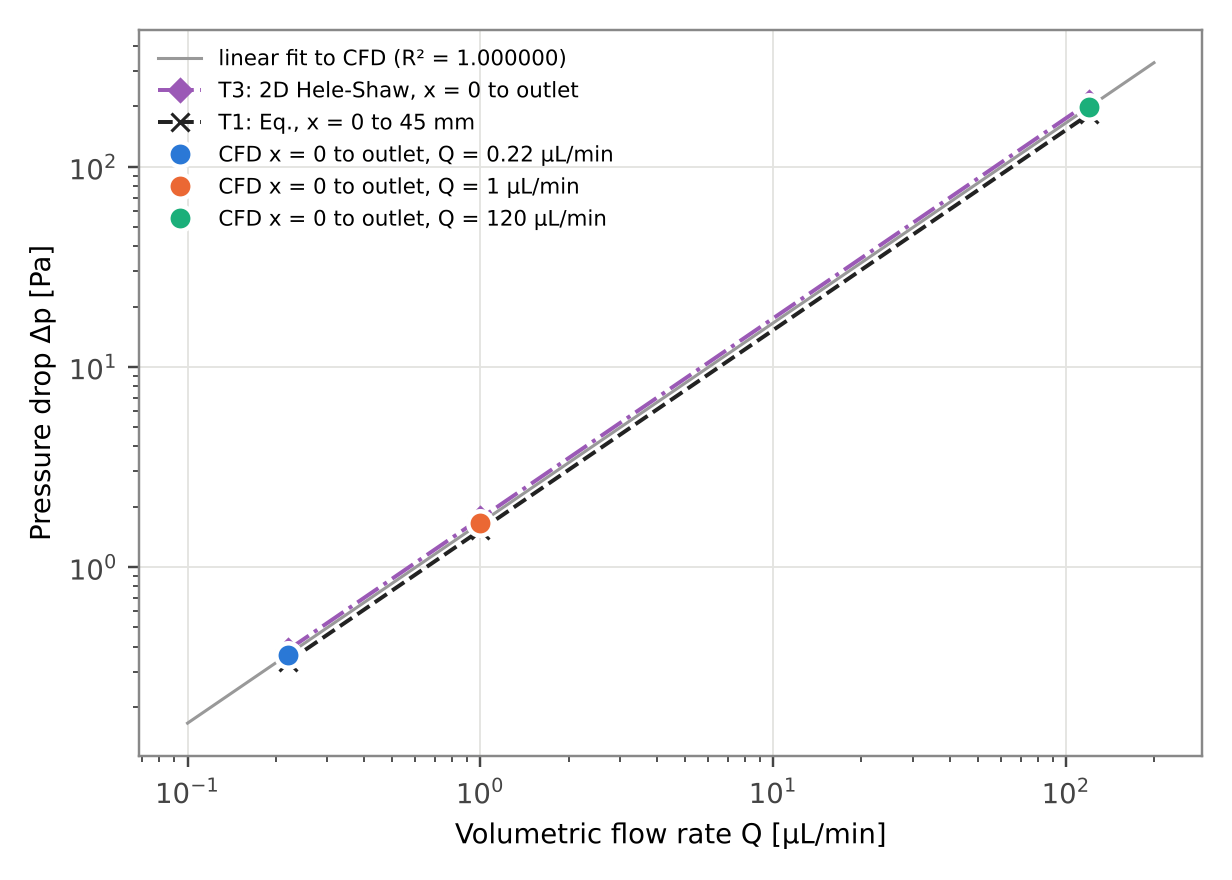
\includegraphics[width=\linewidth]{Fig06_pressure_drop_vs_Q.png}
\caption{Pressure drop against $Q$.}\label{fig:dp_Q}
\end{subfigure}
\caption{Flow-rate scaling of the pressure \tagC. (a) The three axial profiles divided by $Q$ collapse to within \SI{0.02}{\percent}; T3 lies about \SI{5}{\percent} above. (b) The pressure drop from $x=0$ to the outlet is proportional to $Q$ over a factor of 545. The T1 points cover only the hyperbolic section and are therefore lower by construction.}
\end{figure}

\paragraph{Local pressure gradient.} The gradient (\cref{fig:dpdx}, \cref{tab:dpdx}) falls from \SI{63}{Pa/m} per \ulmin\ at $x=0$ to a minimum of \SI{8.7}{Pa/m} per \ulmin\ at $x=\SI{43.9}{mm}$, a factor of 7.3, and then rises steeply in the outlet duct. T1 predicts a factor of 10 at $x=\SI{45}{mm}$. The minimum occurs before the end of the hyperbola because the flow already starts to converge towards the outlet; T3 places it at \SI{44.1}{mm}. Along the hyperbolic section the CFD gradient \emph{crosses} the T1 line: it is \SI{3.3}{\percent} above T1 at S1 and \SI{2.7}{\percent} below at S4. By contrast it is 4.6--\SI{5.4}{\percent} below T2 at every station. The variation relative to T1 is the side-wall effect, which weakens as the channel widens. The constant offset relative to T2 is discussed in \cref{sec:val_offset}.

\begin{figure}[htbp]
\centering
\begin{subfigure}[t]{0.49\linewidth}\centering
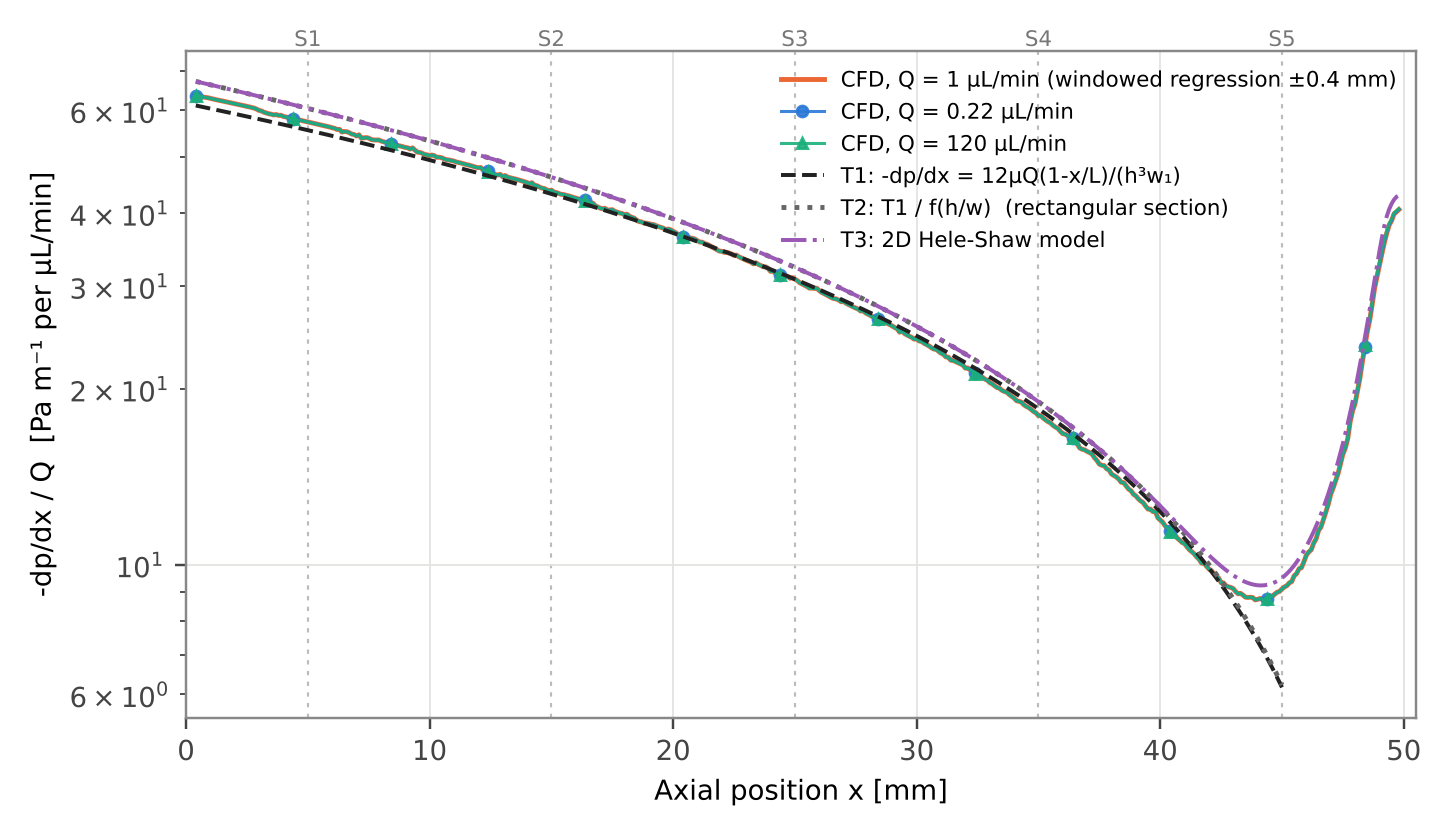
\includegraphics[width=\linewidth]{Fig07_pressure_gradient_vs_x.png}
\caption{Local gradient per unit flow rate.}\label{fig:dpdx}
\end{subfigure}\hfill
\begin{subfigure}[t]{0.49\linewidth}\centering
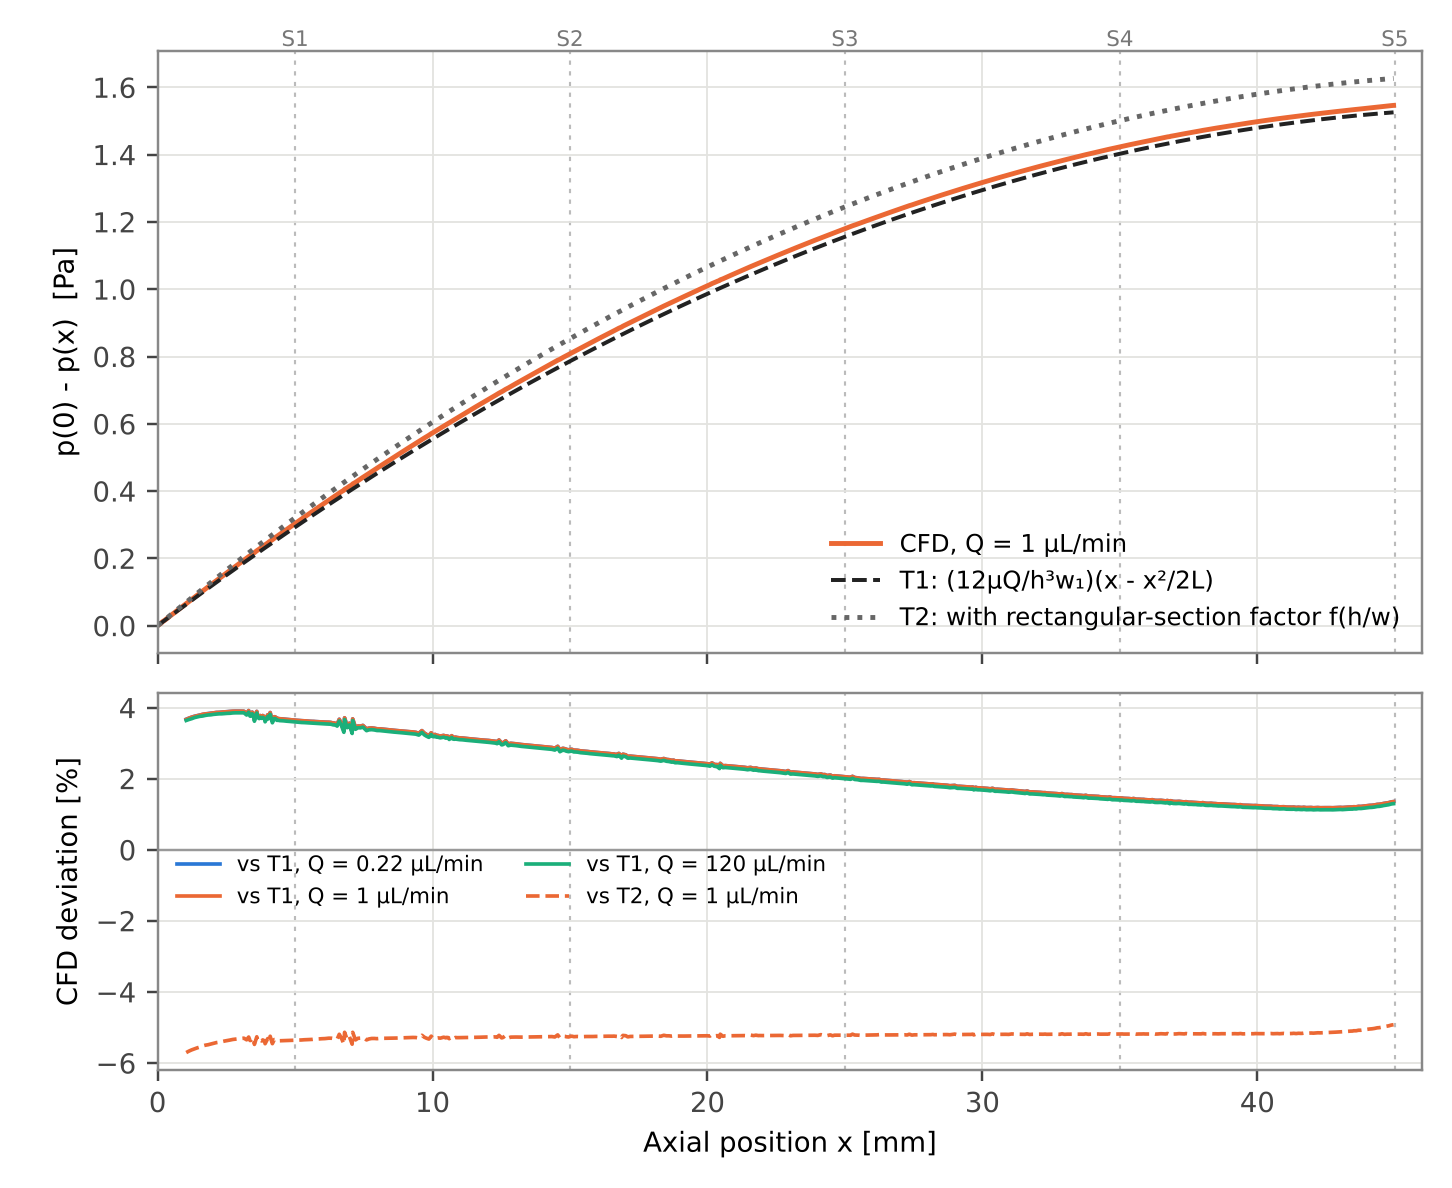
\includegraphics[width=\linewidth]{Fig08_pressure_drop_CFD_vs_theory.png}
\caption{Cumulative drop and deviation from theory.}\label{fig:dp_theory}
\end{subfigure}
\caption{Pressure gradient and cumulative pressure drop \tagC\ against theory \tagT. (a) $|\dd p/\dd x|/Q$ from a $\pm\SI{0.4}{mm}$ least-squares window; the gradient falls linearly with $x$, reaches a minimum at $x\approx\SI{44}{mm}$ and rises in the converging outlet. (b) Top: $p(0)-p(x)$ at \SI{1}{\uLmin} against \cref{eq:th_p}. Bottom: signed deviation from T1 (the three flow rates coincide) and from T2. Over 0--\SI{45}{mm} the CFD is \SI{1.4}{\percent} above T1 and \SI{4.9}{\percent} below T2.}
\end{figure}

\begin{table}[htbp]
\centering
\caption{Pressure gradient at the stations, \SI{1}{\uLmin} (other flow rates identical to within \SI{0.1}{\percent}). T1 and T2 do not apply at S5.}
\label{tab:dpdx}
\small
\begin{tabular}{@{}lcccccc@{}}
\toprule
Station & $h/w$ & $-\dd p/\dd x$ CFD & T1 & Dev.\ vs T1 & T2 & Dev.\ vs T2\\
 & & [Pa/m] & [Pa/m] & [\%] & [Pa/m] & [\%]\\
\midrule
S1 & 0.1305 & 57.32 & 55.49 & $+3.30$ & 60.46 & $-5.20$\\
S2 & 0.1015 & 43.81 & 43.16 & $+1.51$ & 46.11 & $-4.98$\\
S3 & 0.0725 & 30.83 & 30.83 & $+0.01$ & 32.30 & $-4.56$\\
S4 & 0.0435 & 18.00 & 18.50 & $-2.68$ & 19.02 & $-5.35$\\
S5 & 0.0145 & 9.09 & 6.17 & $+47.4$ & 6.22 & $+46.1$\\
\bottomrule
\end{tabular}
\end{table}

\begin{table}[htbp]
\centering
\caption{Pressure summary \tagC/\tagT. CFD values are axial gauge pressures. T1 covers only the hyperbolic section; T3 includes the outlet transition.}
\label{tab:pressure_summary}
\small
\begin{tabular}{@{}lccc@{}}
\toprule
Quantity & \SI{0.22}{\uLmin} & \SI{1}{\uLmin} & \SI{120}{\uLmin}\\
\midrule
$p(x=0)$, CFD [Pa] & 0.3647 & 1.6574 & 198.93\\
$\Delta p_{0-45}$, CFD [Pa] & 0.3404 & 1.5468 & 185.59\\
$\Delta p_{0-45}$, T1 [Pa] & 0.3358 & 1.5260 & 183.19\\
$\Delta p_{0-45}$, T2 [Pa] & 0.3580 & 1.6267 & 195.28\\
CFD vs T1 / vs T2 [\%] & $+1.37$ / $-4.91$ & $+1.37$ / $-4.91$ & $+1.31$ / $-4.97$\\
$\Delta p_{0-\mathrm{outlet}}$, CFD / T3 [Pa] & 0.3646 / 0.3845 & 1.6569 / 1.7475 & 198.88 / 209.78\\
CFD vs T3 [\%] & $-5.18$ & $-5.18$ & $-5.20$\\
\bottomrule
\end{tabular}
\end{table}

\section{Wall shear stress along the axis}
\label{sec:val_shear}

\Cref{fig:tau_axis} shows the axial wall shear at \SI{1}{\uLmin} against T1, T2 and T3. The CFD decreases almost linearly from \SI{4.62}{mPa} per \ulmin\ at $x=0$ to a minimum of \SI{0.630}{mPa} per \ulmin\ at $x=\SI{44.0}{mm}$ (T3: \SI{44.1}{mm}), then rises to \SI{3.03}{mPa} per \ulmin\ in the outlet duct. \Cref{tab:shear_stations} gives the station values for all three flow rates.

\begin{figure}[htbp]
\centering
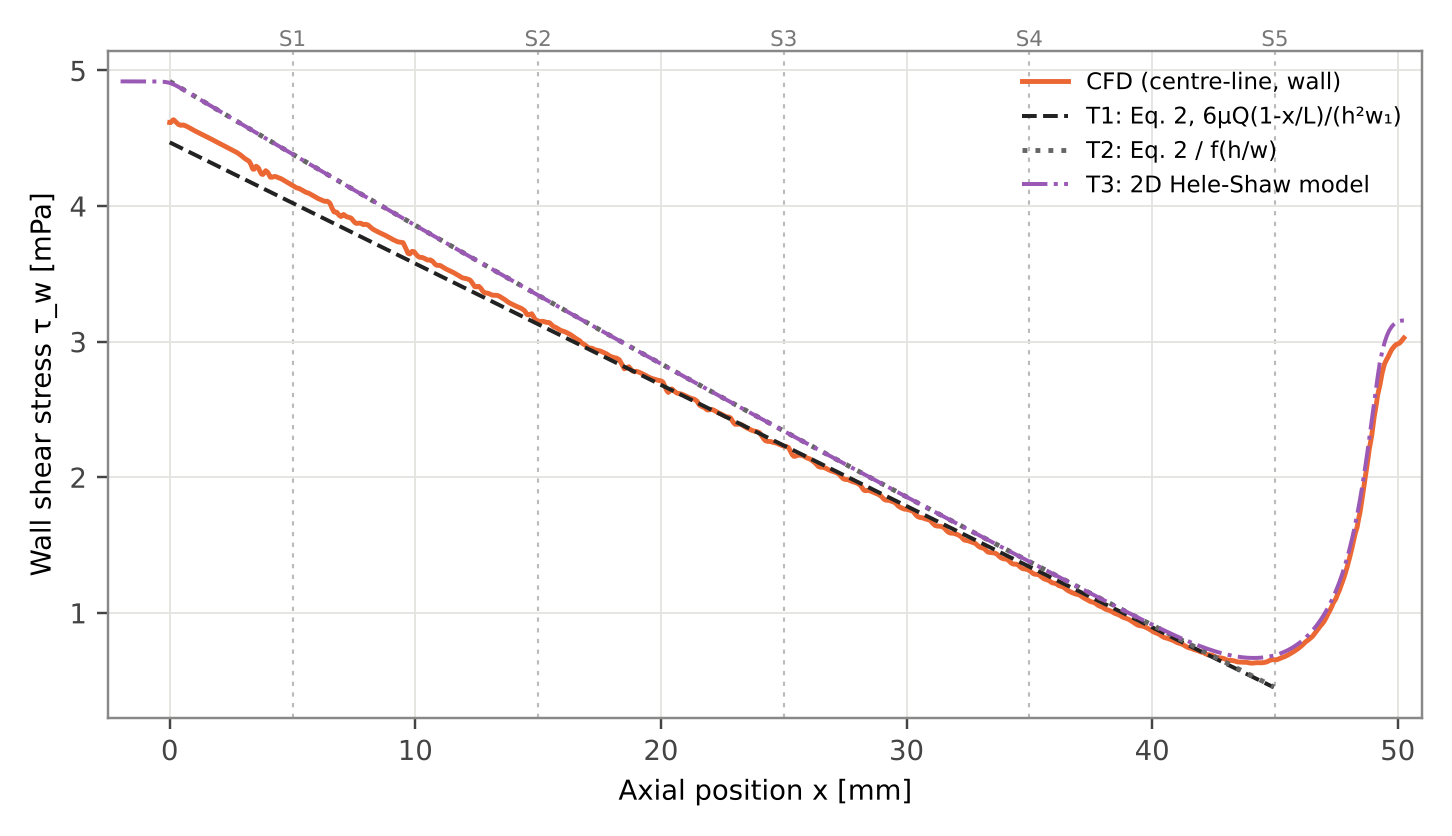
\includegraphics[width=0.88\linewidth]{Fig11_wall_shear_vs_x_Q1.png}
\caption{Wall shear on the axis at \SI{1}{\uLmin}: CFD \tagC\ against Eq.~2 (T1), the side-wall-corrected theory (T2) and the 2D model (T3) \tagT. The CFD lies above T1 near the inlet and below it near S4, and runs parallel to T2/T3 about \SI{5}{\percent} lower. Beyond $x\approx\SI{42}{mm}$ the CFD and T3 rise away from T1.}
\label{fig:tau_axis}
\end{figure}

\begin{table}[htbp]
\centering
\caption{Axial wall shear at the stations compared with Eq.~2 (T1) for all flow rates. Signed deviation $=\tau_{\mathrm{CFD}}/\tau_{T1}-1$. Deviations from T2 and T3 are given for reference.}
\label{tab:shear_stations}
\small
\begin{tabular}{@{}llccccc@{}}
\toprule
Station & $Q$ [\ulmin] & $\taw$ CFD [Pa] & $\taw$ T1 [Pa] & Dev.\ T1 [\%] & Dev.\ T2 [\%] & Dev.\ T3 [\%]\\
\midrule
S1 & 0.22 & \num{9.140e-4} & \num{8.852e-4} & $+3.25$ & $-5.24$ & $-5.24$\\
S2 & 0.22 & \num{6.935e-4} & \num{6.885e-4} & $+0.72$ & $-5.72$ & $-5.71$\\
S3 & 0.22 & \num{4.908e-4} & \num{4.918e-4} & $-0.21$ & $-4.77$ & $-4.75$\\
S4 & 0.22 & \num{2.888e-4} & \num{2.951e-4} & $-2.12$ & $-4.80$ & $-4.79$\\
S5 & 0.22 & \num{1.441e-4} & \num{9.836e-5} & $+46.47$ & n/a & $-4.87$\\
\addlinespace
S1 & 1 & \num{4.154e-3} & \num{4.023e-3} & $+3.25$ & $-5.24$ & $-5.23$\\
S2 & 1 & \num{3.152e-3} & \num{3.129e-3} & $+0.72$ & $-5.72$ & $-5.71$\\
S3 & 1 & \num{2.230e-3} & \num{2.235e-3} & $-0.21$ & $-4.77$ & $-4.75$\\
S4 & 1 & \num{1.313e-3} & \num{1.341e-3} & $-2.12$ & $-4.81$ & $-4.79$\\
S5 & 1 & \num{6.547e-4} & \num{4.470e-4} & $+46.47$ & n/a & $-4.87$\\
\addlinespace
S1 & 120 & \num{4.988e-1} & \num{4.830e-1} & $+3.29$ & $-5.21$ & $-5.20$\\
S2 & 120 & \num{3.784e-1} & \num{3.756e-1} & $+0.72$ & $-5.72$ & $-5.71$\\
S3 & 120 & \num{2.677e-1} & \num{2.683e-1} & $-0.22$ & $-4.78$ & $-4.77$\\
S4 & 120 & \num{1.575e-1} & \num{1.610e-1} & $-2.14$ & $-4.83$ & $-4.81$\\
S5 & 120 & \num{7.859e-2} & \num{5.366e-2} & $+46.46$ & n/a & $-4.87$\\
\bottomrule
\end{tabular}
\end{table}

\paragraph{Error metrics.} Over the central region $2\le x\le\SI{40}{mm}$ (about 570 points), the CFD deviates from the three theories as follows (identical at all $Q$ to within \SI{0.02}{\percent}):

\begin{center}
\small
\begin{tabular}{@{}lccc@{}}
\toprule
Metric (2--\SI{40}{mm}, \SI{1}{\uLmin}) & vs T1 & vs T2 & vs T3\\
\midrule
RMSE [mPa] & 0.064 & 0.156 & 0.156\\
Normalised RMSE (RMSE / mean theory) [\%] & 2.45 & 5.62 & 5.61\\
Mean absolute percentage error [\%] & 1.79 & 5.16 & 5.16\\
Maximum absolute percentage error [\%] & 4.04 & 6.47 & 6.46\\
\bottomrule
\end{tabular}
\end{center}

\noindent On these metrics alone, Eq.~2 (T1) would appear to be the best theory. The next two figures show that this is misleading.

\begin{figure}[htbp]
\centering
\begin{subfigure}[t]{0.49\linewidth}\centering
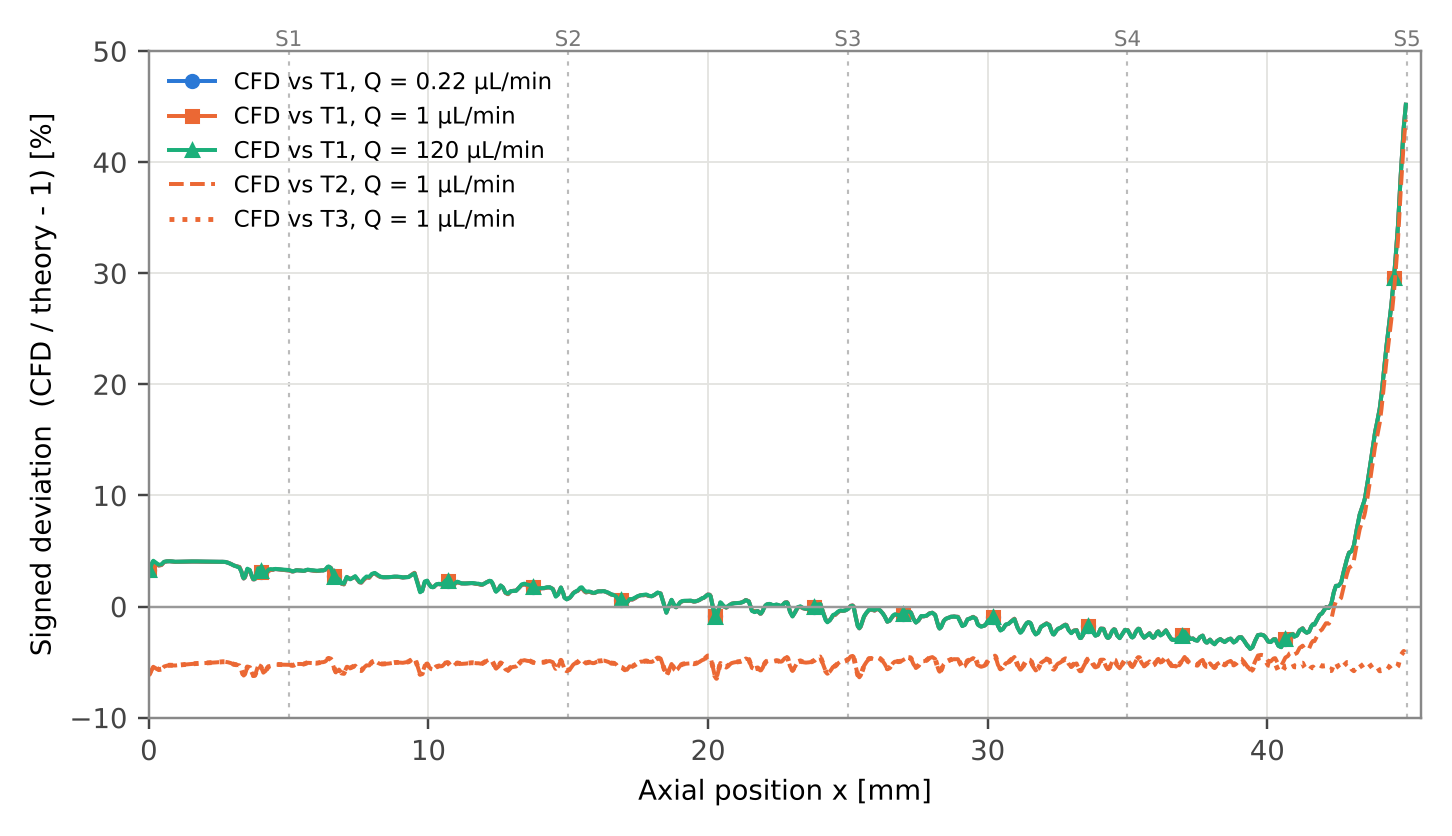
\includegraphics[width=\linewidth]{Fig15_wall_shear_percentage_deviation.png}
\caption{Signed deviation along $x$.}\label{fig:tau_dev}
\end{subfigure}\hfill
\begin{subfigure}[t]{0.49\linewidth}\centering
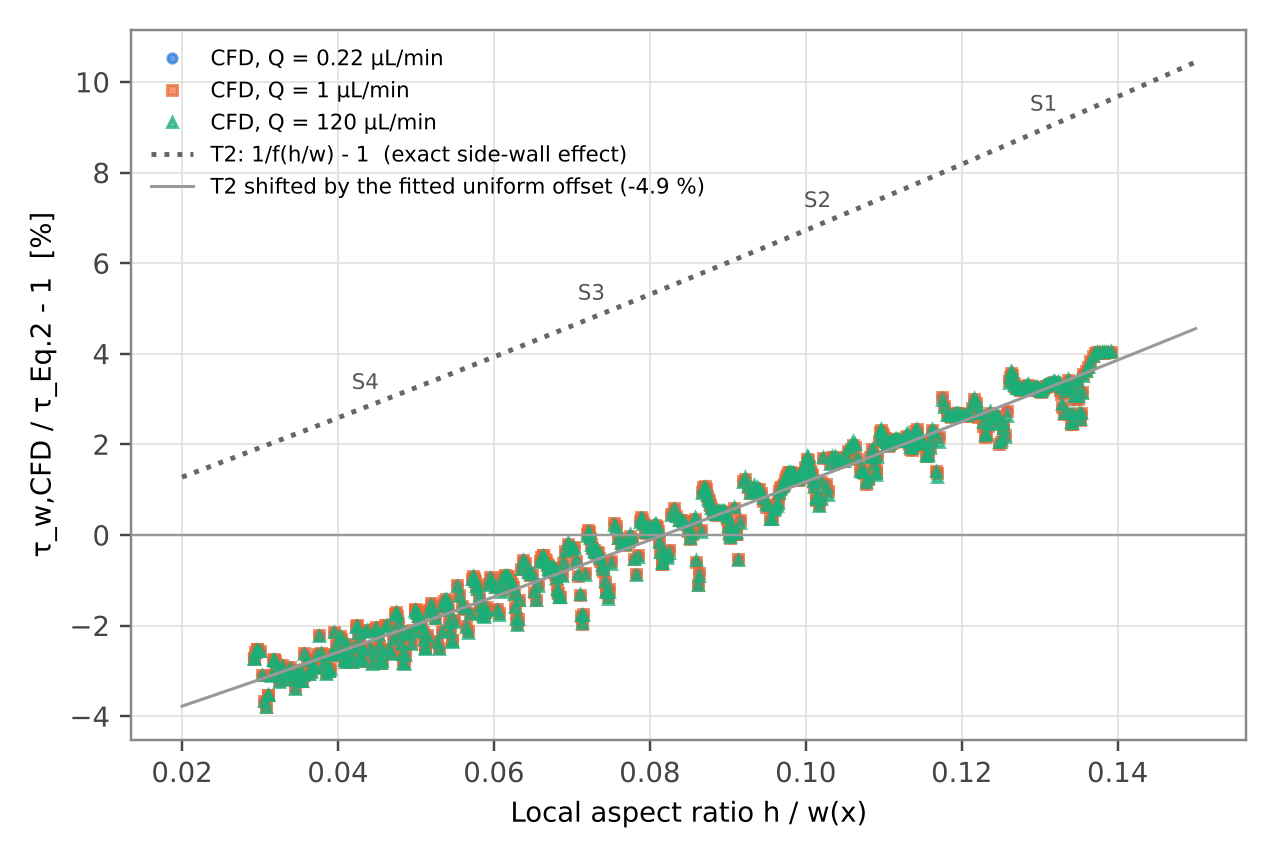
\includegraphics[width=\linewidth]{Fig16_shear_deviation_vs_aspect_ratio.png}
\caption{Deviation from Eq.~2 against $h/w$.}\label{fig:tau_hw}
\end{subfigure}
\caption{Structure of the deviation of the CFD shear from theory \tagC. (a) Against Eq.~2 the deviation runs from about \SI{+4}{\percent} at the inlet through zero at $x\approx\SI{23}{mm}$ to $-2$ to \SI{-3}{\percent} at S4--\SI{40}{mm}, then rises steeply to \SI{+46}{\percent} at S5. Against T2 it is a near-constant \SI{-5.2(4)}{\percent}; against T3 it stays at \SI{-5}{\percent} including S5. (b) Points: CFD between $x=2$ and \SI{40}{mm}. They follow a line parallel to the exact side-wall correction $1/f-1$ (slope difference only $-0.026$ per unit $h/w$), shifted by \SI{-4.9}{\percent}.}
\end{figure}

\paragraph{Why the deviation from Eq.~2 is systematic.} \Cref{fig:tau_hw} plots the deviation from Eq.~2 against the local aspect ratio. If the only error in Eq.~2 were the neglect of side walls, the points would lie on the T2 curve $1/f(h/w)-1\approx0.63\,h/w$. They lie on a line with exactly that slope (residual slope $-0.026$ per unit $h/w$, scatter \SI{\pm0.36}{\percent}), shifted down by \SI{4.9}{\percent}. The 3D CFD therefore captures the side-wall drag that Eq.~2 omits, with the correct coefficient. On top of that it carries a uniform offset. Near the inlet the two effects partly cancel (\SI{+9}{\percent} side-wall drag, \SI{-5}{\percent} offset, net \SI{+3.3}{\percent}), and near S3 they cancel exactly. The small RMSE against Eq.~2 is therefore a coincidence of two errors, not a validation of Eq.~2.

\paragraph{Linearity.} A straight line fitted to the CFD over 5--\SI{40}{mm} has $R^2=0.9996$, but it reaches zero at $x=\SI{48.8}{mm}$ rather than at $L=\SI{50}{mm}$ and departs from the data by up to \SI{5}{\percent}. The same fit applied to T2 also gives \SI{48.8}{mm}, so the curvature is physical. The side walls raise the shear most where the channel is narrowest, which steepens the decrease. The shear is linear in $x$ to within about $\pm\SI{4}{\percent}$ over the central region.

\section{Transverse distribution of the wall shear}
\label{sec:val_transverse}

\Cref{fig:transverse} shows the floor shear across the width at the five stations, and its normalised form. At S1--S4 the profile is a flat plateau (variation 0.1--\SI{0.7}{\percent} over the central half) that drops near each side wall. In absolute units the drop-off zone has the same thickness at every station. Plotted against the distance from the side wall (\cref{fig:sidewall}), the S1--S4 profiles collapse onto one curve, as \cref{eq:th_delta} predicts: the layer scales with $h$, not with $w$. At S5 there is no plateau. The shear falls continuously from the axis to near zero in the corners, because S5 is the corner of the planform. T3 reproduces this dome shape (\cref{fig:T3}).

\begin{figure}[htbp]
\centering
\begin{subfigure}[t]{0.49\linewidth}\centering
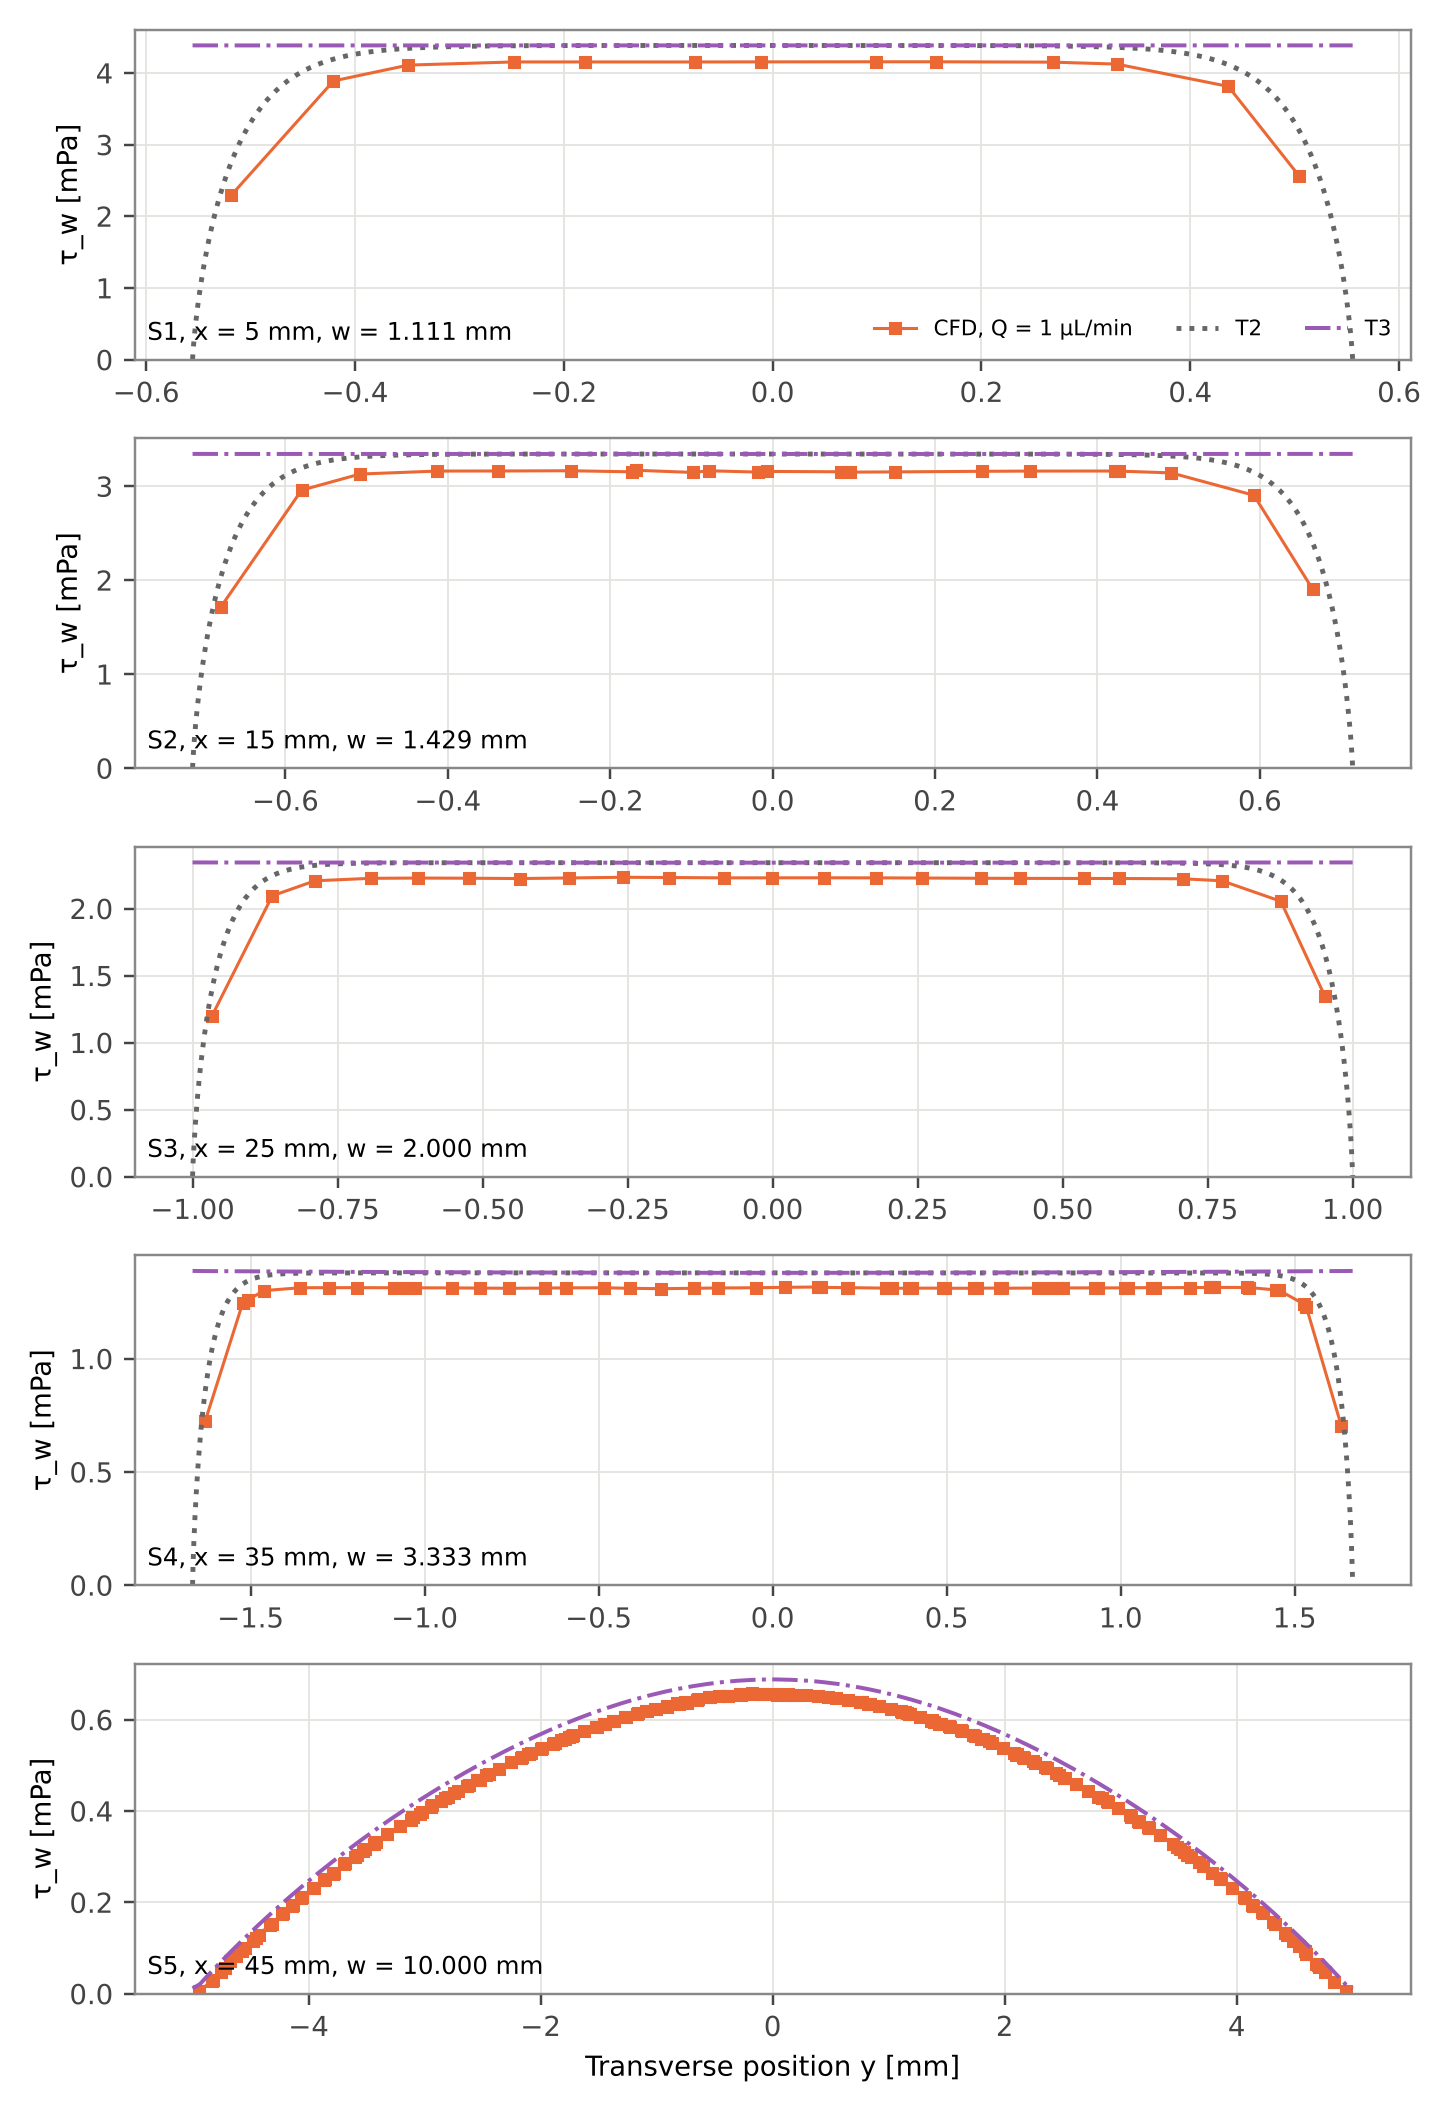
\includegraphics[width=\linewidth]{Fig22_transverse_shear_all_sections.png}
\caption{Profiles at S1--S5.}
\end{subfigure}\hfill
\begin{subfigure}[t]{0.49\linewidth}\centering
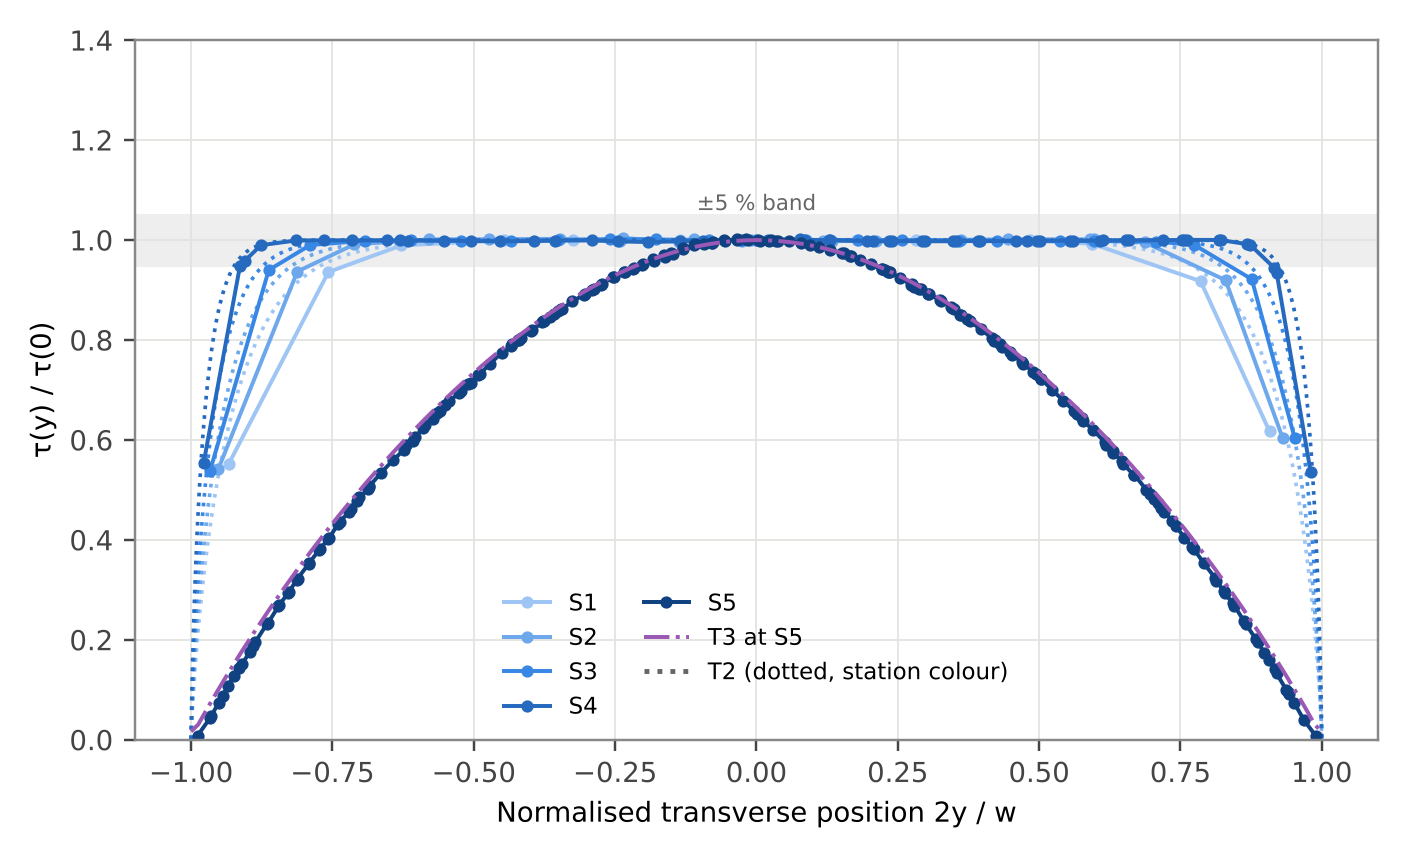
\includegraphics[width=\linewidth]{Fig24_transverse_shear_normalised.png}
\caption{Normalised by axis value and half-width.}
\end{subfigure}
\caption{Floor shear across the width at \SI{1}{\uLmin} \tagC. Each point is the mean of the coincident floor and lid wall nodes. (a) At S1--S4 a flat plateau is bounded by side-wall layers of about \SI{0.15}{mm}; at S5 the profile is a dome. (b) In the normalised coordinate $2y/w$ the plateau widens downstream, because the layer has a fixed thickness while the channel widens.}
\label{fig:transverse}
\end{figure}

\begin{figure}[htbp]
\centering
\begin{subfigure}[t]{0.49\linewidth}\centering
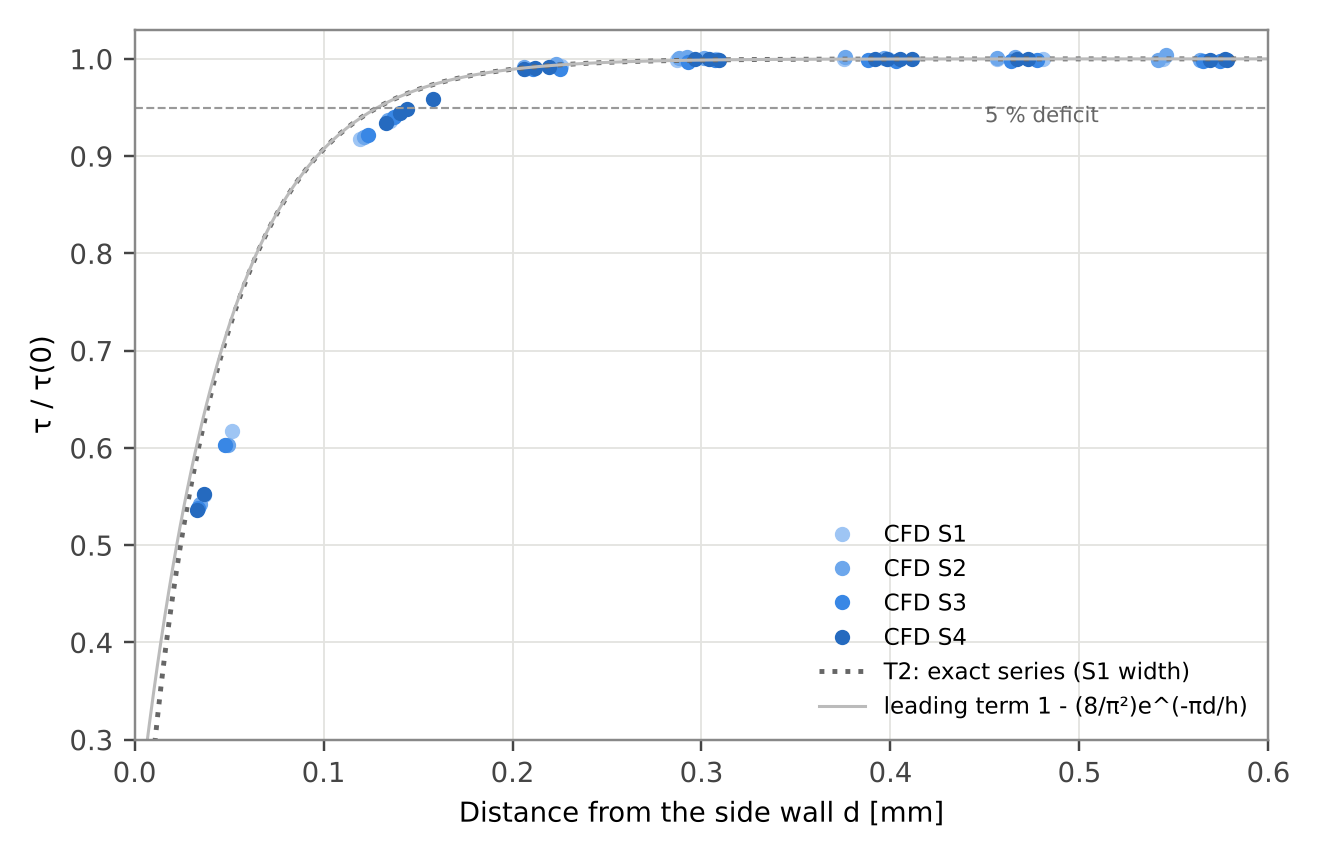
\includegraphics[width=\linewidth]{Fig25_sidewall_layer_collapse.png}
\caption{Side-wall layer collapse.}\label{fig:sidewall}
\end{subfigure}\hfill
\begin{subfigure}[t]{0.49\linewidth}\centering
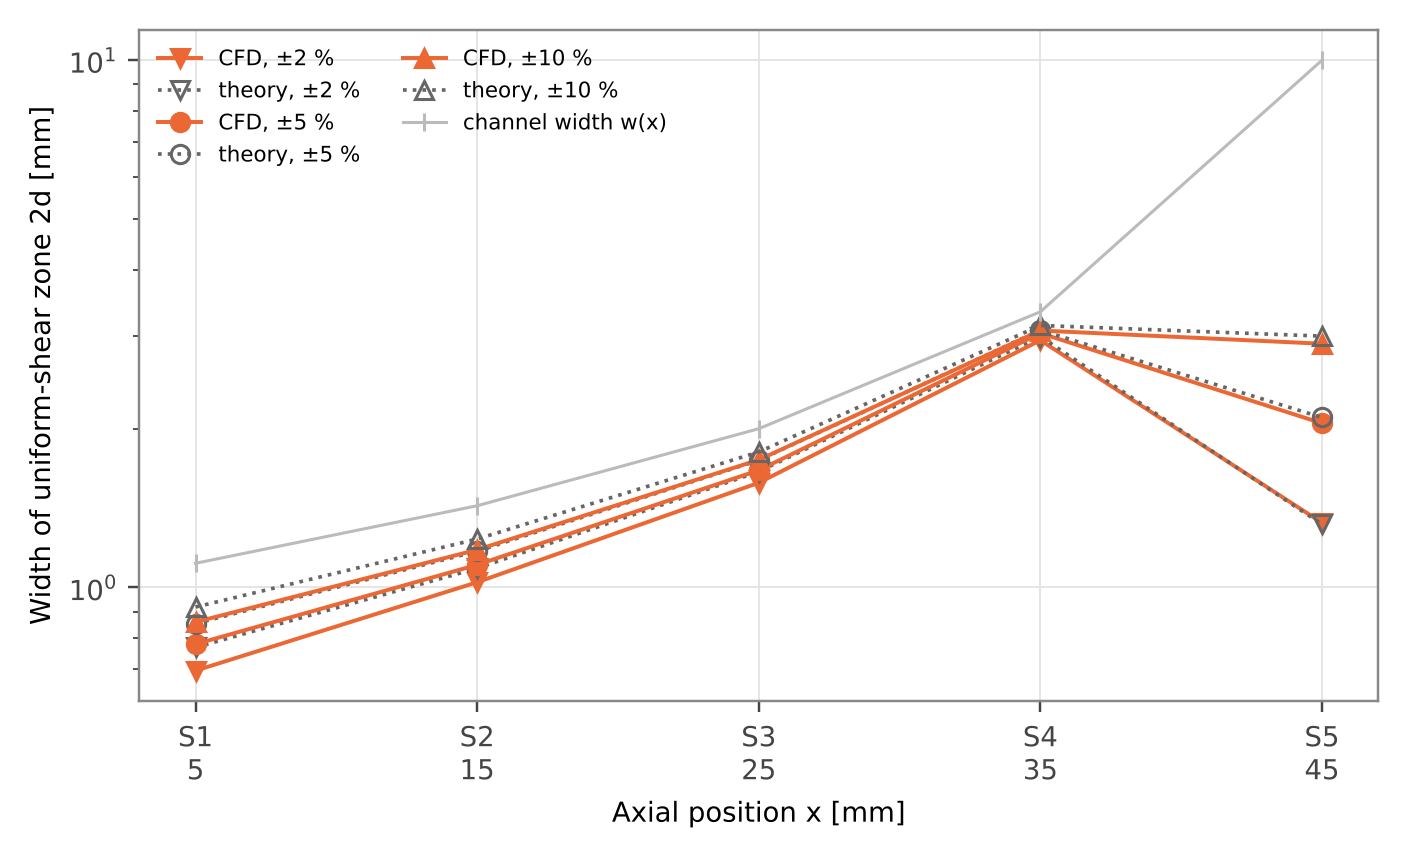
\includegraphics[width=\linewidth]{Fig26_uniform_zone_width_vs_x.png}
\caption{Uniform-zone width $2d$ and tolerance.}\label{fig:uniform}
\end{subfigure}
\caption{(a) Floor shear against the distance from the side wall at S1--S4 \tagC. The profiles collapse; the theoretical \SI{5}{\percent} point is \SI{0.129}{mm} from the wall, and the CFD wall nodes are \SIrange{0.08}{0.10}{mm} apart. (b) Width $2d$ of the central band with $|\tau(y)/\tau(0)-1|\le\varepsilon$ for $\varepsilon=2$, 5 and \SI{10}{\percent} (other flow rates differ by less than \SI{0.002}{mm}). Theory: T2 at S1--S4, T3 at S5.}
\end{figure}

\Cref{tab:uniform} quantifies the uniform zone. At S1--S4 the CFD half-width is 0.009--\SI{0.031}{mm} smaller than the theory evaluated at the same node positions. The CFD side-wall layer is \SIrange{0.149}{0.166}{mm}, against \SI{0.129}{mm} from theory. Both differences are below the \SIrange{0.08}{0.10}{mm} spacing of the exported wall nodes (\cref{tab:transverse_nodes}), so the exports confirm the theoretical layer to within their resolution but cannot resolve it more finely. The uniform fraction grows from \SI{70}{\percent} of the width at S1 to \SI{91}{\percent} at S4, and collapses to \SI{20}{\percent} at S5, in agreement with T3 (\SI{2.10}{mm} against \SI{2.05}{mm} for $2d$). The flow rate has no effect: $d$ differs by at most \SI{0.002}{mm} between 0.22 and \SI{120}{\uLmin}. The tolerance matters little at S4 (\SIrange{-3}{+1}{\percent} change in width between $\pm2$ and $\pm\SI{10}{\percent}$) but a great deal at S5 (\SIrange{-35}{+42}{\percent}), where there is no plateau.

\begin{table}[htbp]
\centering
\caption{Uniform-shear half-width $d$ at $\pm\SI{5}{\percent}$ \tagC, with theory \tagT\ (T2 at S1--S4, T3 at S5) and the sensitivity of $2d$ to the tolerance (\SI{1}{\uLmin}). Side layer $=w/2-d$.}
\label{tab:uniform}
\small
\resizebox{\linewidth}{!}{%
\begin{tabular}{@{}lcccccccc@{}}
\toprule
Station & $w/2$ & $d$ (0.22/1/120) & $2d/w$ & $d$ theory & side layer & side layer & $2d$ at $\pm2/5/10\,\%$ & $2d/w$ at\\
 & [mm] & [mm] & [\%] & [mm] & CFD [mm] & theory [mm] & [mm] & $\pm2/5/10\,\%$\\
\midrule
S1 & 0.556 & 0.390/0.390/0.389 & 70.3 & 0.427 & 0.165 & 0.129 & 0.695/0.781/0.860 & 63/70/77\\
S2 & 0.714 & 0.552/0.552/0.552 & 77.3 & 0.586 & 0.162 & 0.129 & 1.023/1.104/1.179 & 72/77/83\\
S3 & 1.000 & 0.834/0.834/0.834 & 83.4 & 0.871 & 0.166 & 0.129 & 1.579/1.668/1.746 & 79/83/87\\
S4 & 1.667 & 1.518/1.518/1.517 & 91.1 & 1.538 & 0.149 & 0.129 & 2.943/3.035/3.071 & 88/91/92\\
S5 & 5.000 & 1.024/1.024/1.025 & 20.5 & 1.050 & 3.976 & 3.950 & 1.326/2.048/2.899 & 13/20/29\\
\bottomrule
\end{tabular}}
\end{table}

\begin{table}[htbp]
\centering
\caption{Cross-section exports at \SI{1}{\uLmin}: consistency with the axial export and resolution near the side walls \tagC.}
\label{tab:transverse_nodes}
\small
\begin{tabular}{@{}lcccccc@{}}
\toprule
Station & Points & Wall nodes & $\tau(0)$ section & $\tau$ axial export & Floor--lid spread & Node spacing at\\
 & & (side/corner) & [mPa] & [mPa] & mean/max [\%] & side wall [mm]\\
\midrule
S1 & 171 & 34 (8) & 4.1542 & 4.1537 & 0.64 / 4.3 & 0.083\\
S2 & 207 & 41 (7) & 3.1571 & 3.1516 & 0.82 / 4.9 & 0.086\\
S3 & 267 & 54 (8) & 2.2291 & 2.2303 & 0.12 / 0.6 & 0.090\\
S4 & 457 & 91 (8) & 1.3143 & 1.3125 & 0.51 / 6.6 & 0.104\\
S5 & 1349 & 265 (8) & 0.6556 & 0.6547 & 0.63 / 6.7 & 0.106\\
\bottomrule
\end{tabular}
\end{table}

\section{Velocity field}
\label{sec:val_velocity}

The velocity exports contain $|\vect u|$ at all node heights plotted against $y$. Each section therefore appears as a scatter from zero up to about the mid-plane velocity. The upper envelope approximates the mid-plane profile and slightly underestimates it. At S1--S4 the walls diverge at half-angles of only \ang{0.7}--\ang{6.3}, so $|\vect u|$ exceeds $u_x$ by at most \SI{0.6}{\percent} and can be read as the axial velocity. \Cref{fig:velocity} shows a flat core with a side-wall layer of the same thickness as for the shear, as \cref{eq:th_rect_u} predicts. The peak velocity falls from \SI{0.166}{mm/s} per \ulmin\ at S1 to \SI{0.026}{mm/s} per \ulmin\ at S5, in proportion to $1/[wf(h/w)]$. The highest sampled velocity is \SIrange{1.2}{3.4}{\percent} below the theoretical mid-plane value (\cref{tab:velocity}). The pathlines (\cref{fig:pathlines}) follow the diverging walls without separation and converge smoothly into the outlet, at 1 and at \SI{120}{\uLmin}.

\begin{figure}[htbp]
\centering
\begin{subfigure}[t]{0.49\linewidth}\centering
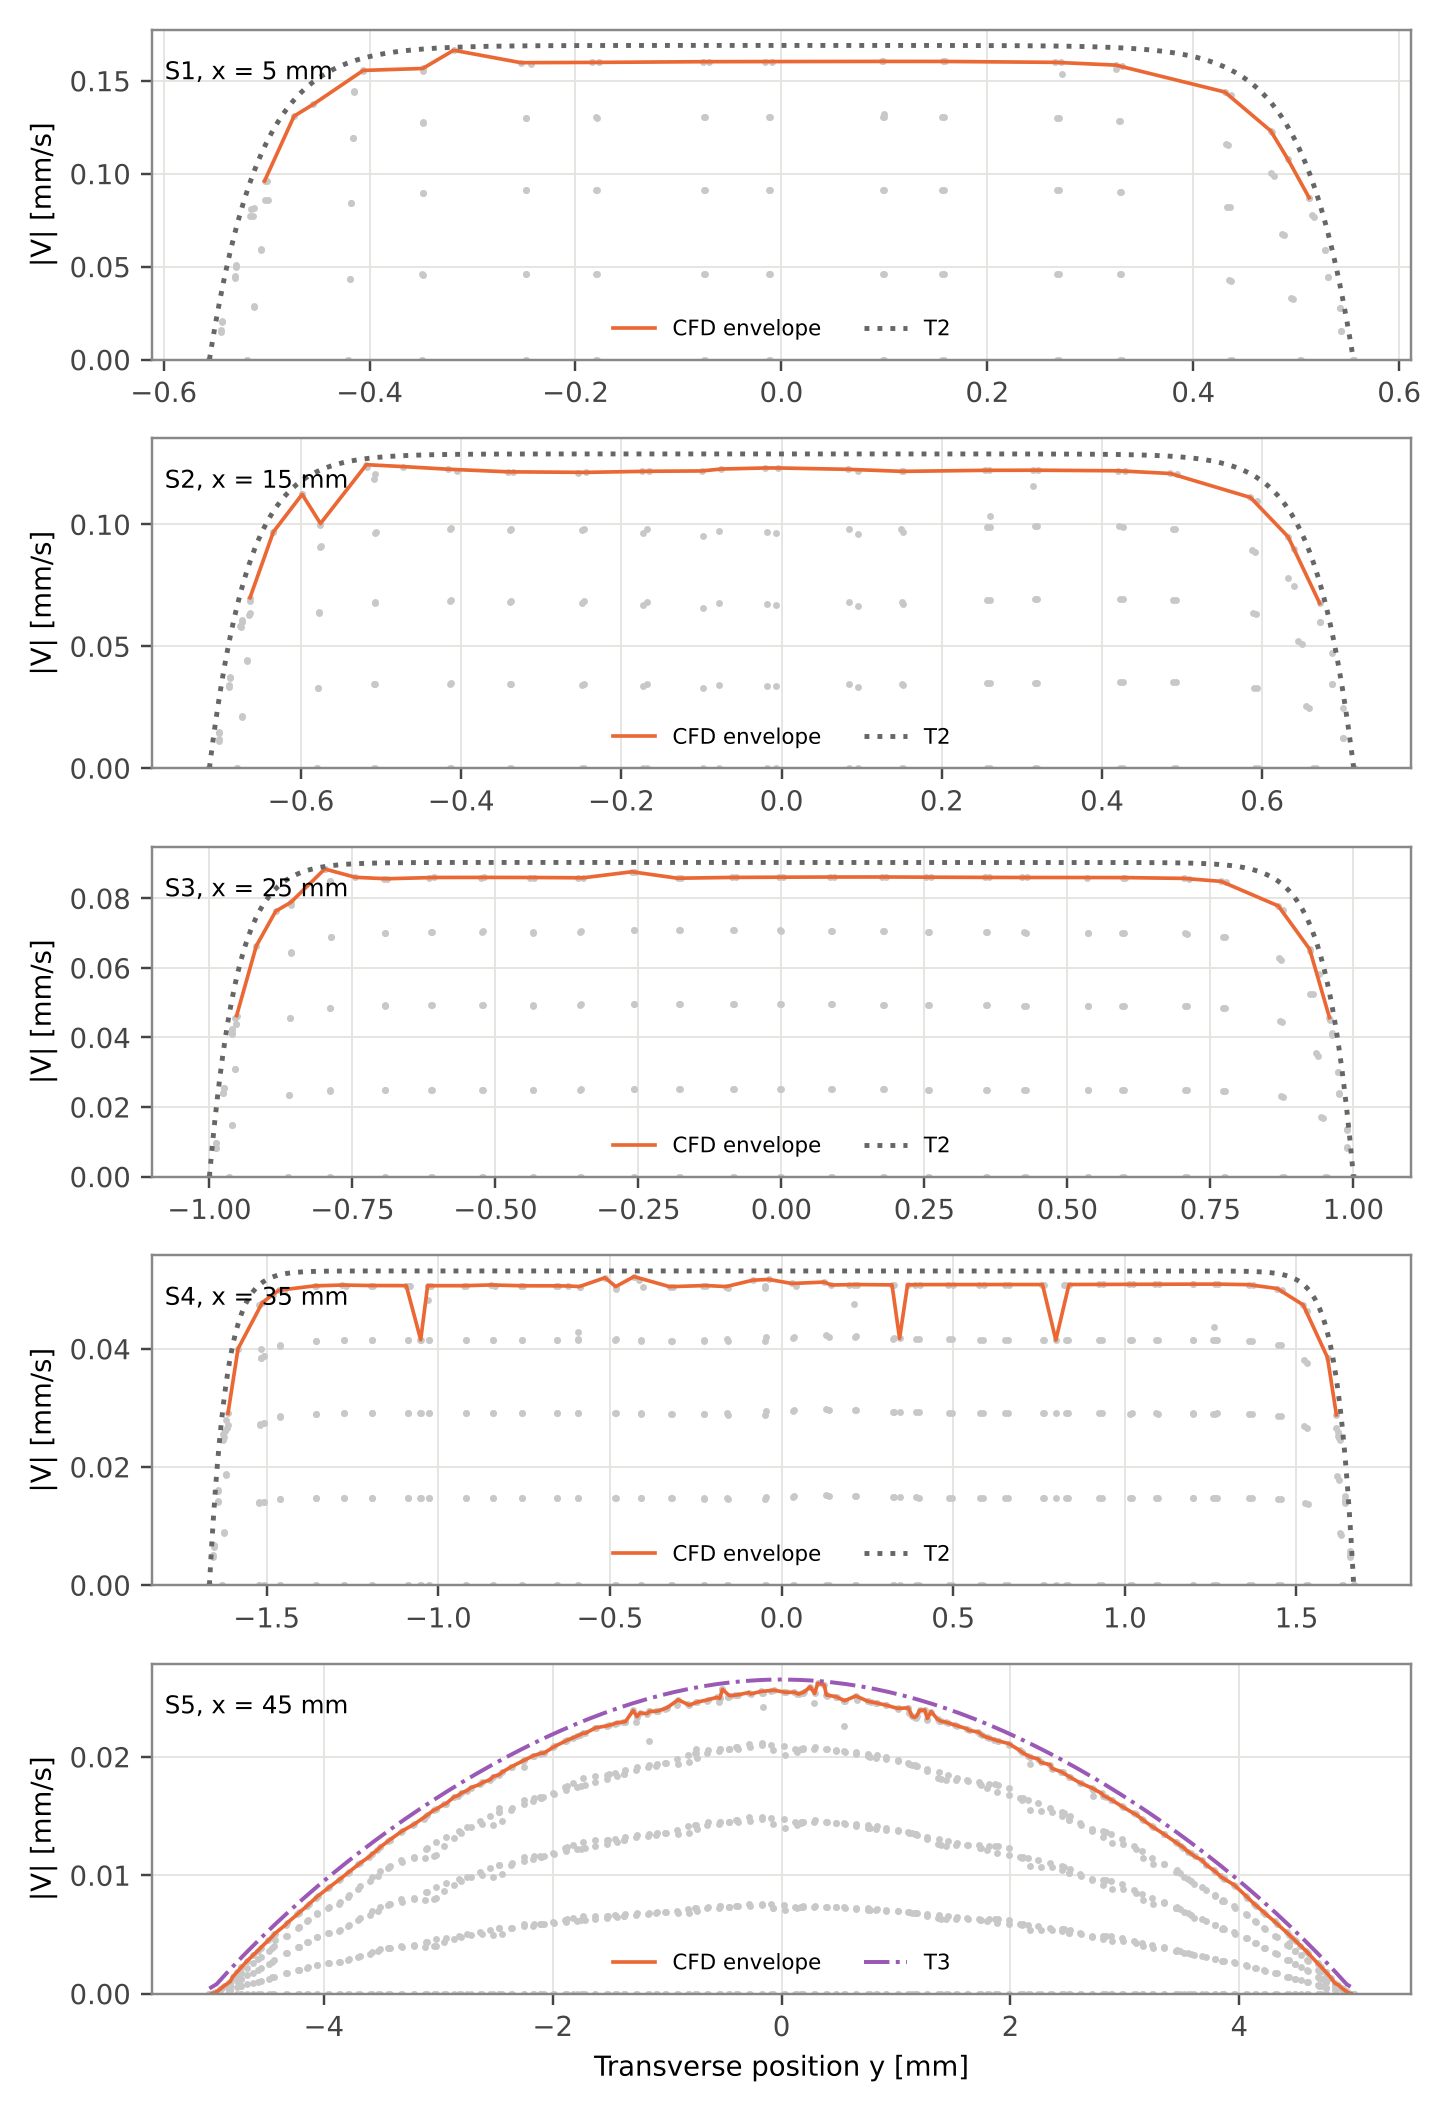
\includegraphics[width=\linewidth]{Fig33_transverse_velocity_all_sections.png}
\caption{Velocity magnitude across the width.}
\end{subfigure}\hfill
\begin{subfigure}[t]{0.49\linewidth}\centering
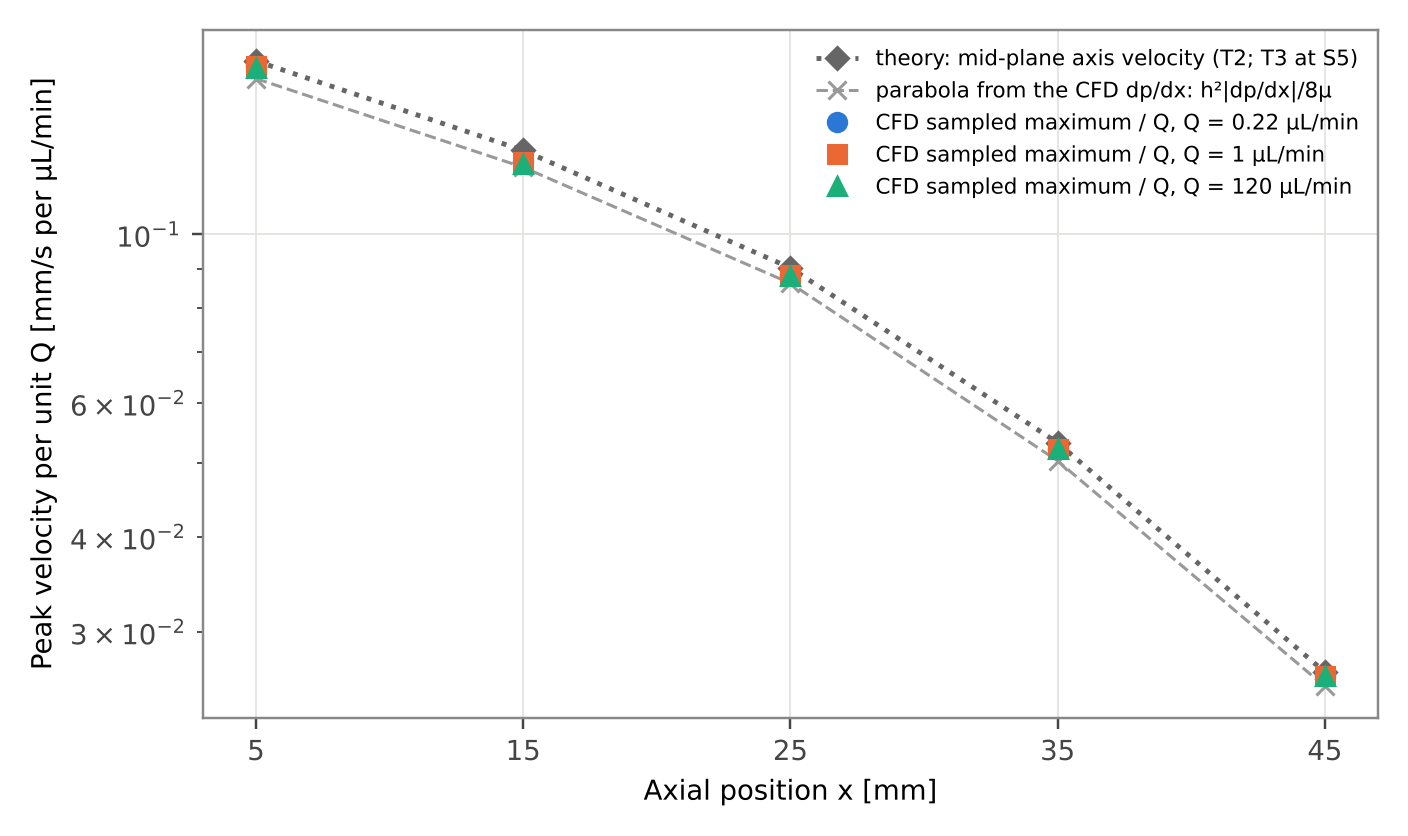
\includegraphics[width=\linewidth]{Fig35_peak_velocity_vs_x.png}
\caption{Peak velocity along the channel.}
\end{subfigure}
\caption{Velocity at the stations \tagC. (a) Nodes at all heights plotted against $y$ (\SI{1}{\uLmin}). The upper envelope is the near-mid-plane profile: a flat core with side-wall layers. (b) Highest sampled $|\vect u|/Q$ against the theoretical mid-plane maximum (T2 at S1--S4, T3 at S5).}
\label{fig:velocity}
\end{figure}

\begin{figure}[htbp]
\centering
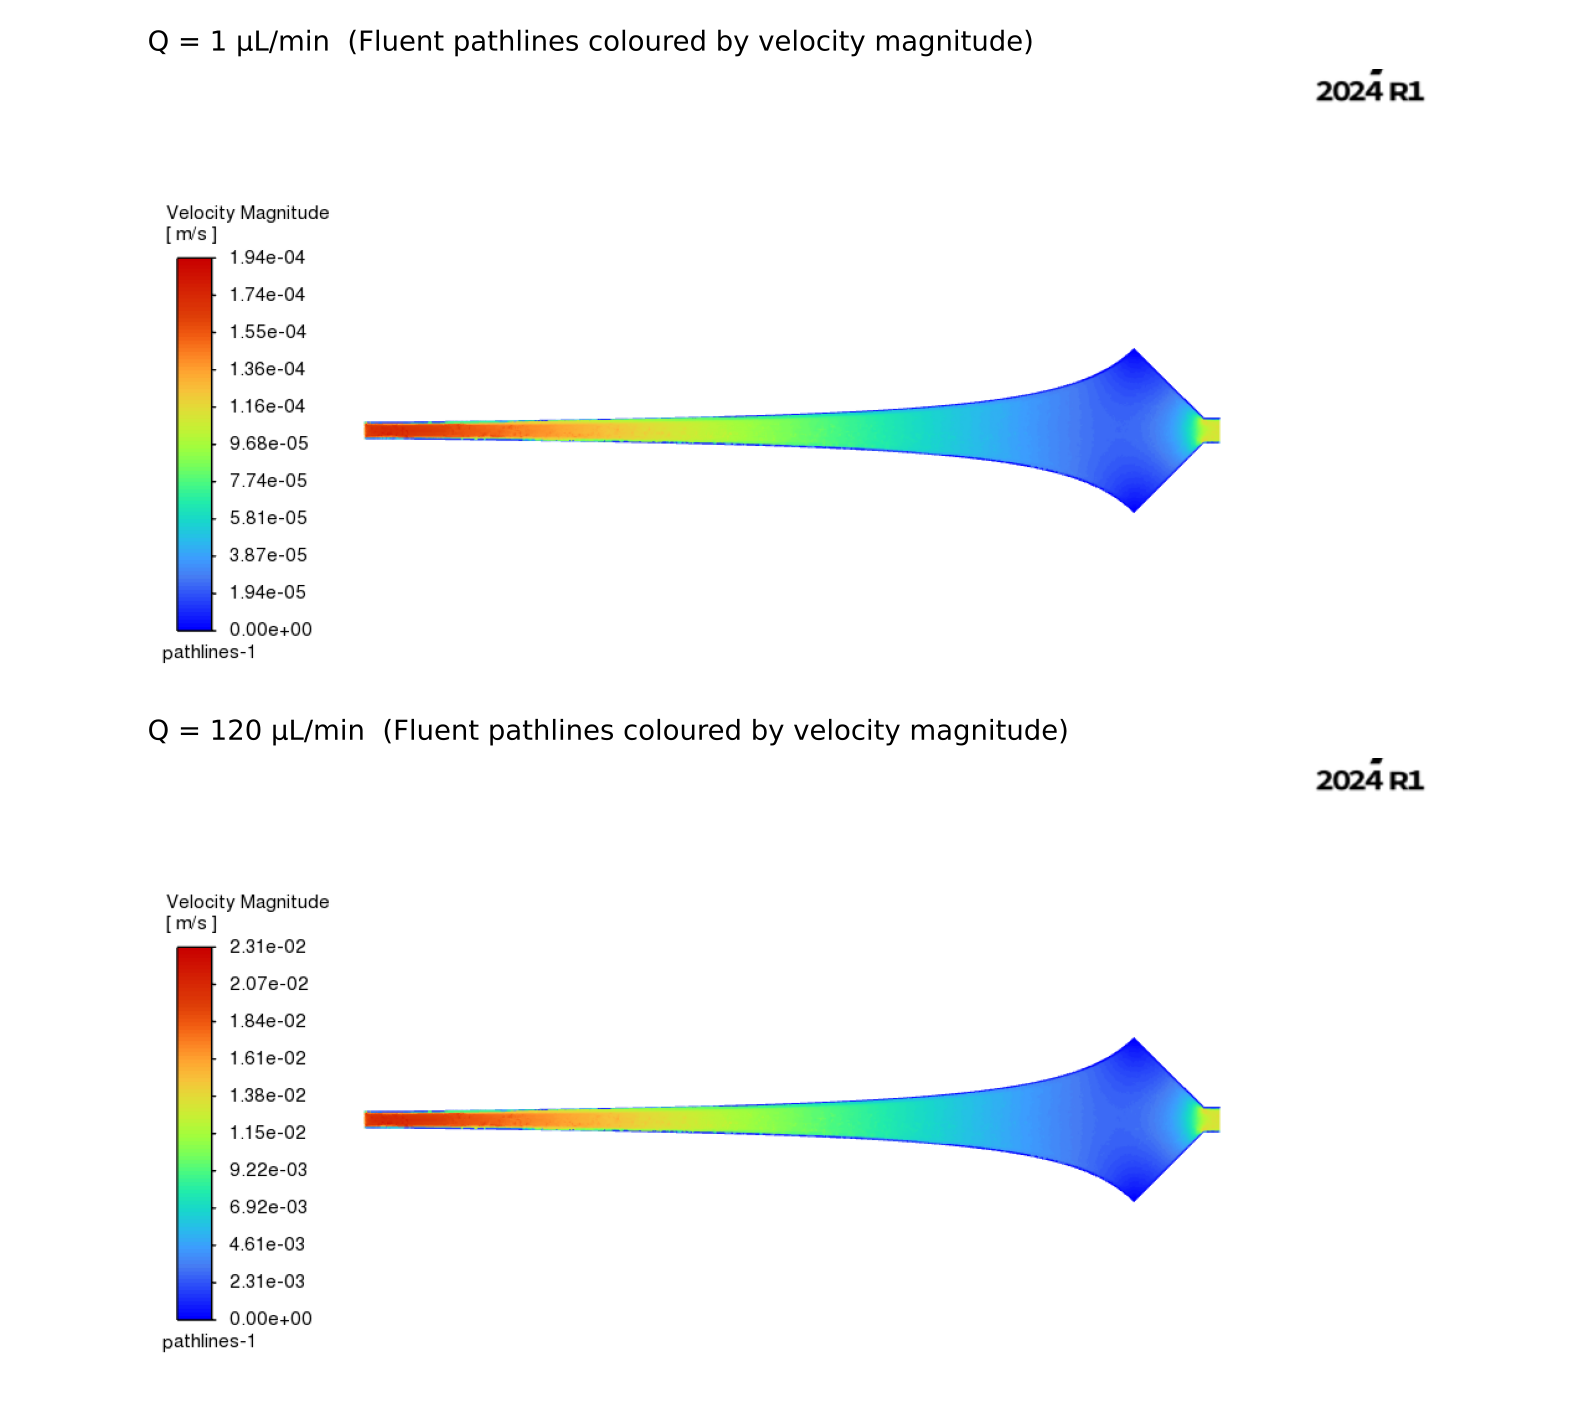
\includegraphics[width=0.75\linewidth]{Fig36_pathlines_Q1_Q120.png}
\caption{Pathlines coloured by velocity magnitude at 1 and \SI{120}{\uLmin} (Fluent images) \tagC. The maximum velocity scales by 119.1 between the two flow rates (Stokes flow: 120). There is no separation or recirculation in the outlet corners.}
\label{fig:pathlines}
\end{figure}

\begin{table}[htbp]
\centering
\caption{Velocity at the stations, \SI{1}{\uLmin}. Theory: T2 mid-plane axis value at S1--S4, T3 at S5. The last column compares the sampled maximum with the parabola implied by the CFD's own pressure gradient, $h^2|\dd p/\dd x|/8\mu$ (\cref{eq:th_umax}).}
\label{tab:velocity}
\small
\begin{tabular}{@{}lccccc@{}}
\toprule
Station & Wall half-angle & Max.\ sampled $|\vect u|$ & Theory mid-plane & Max / theory & Max / $\frac{h^2|\dd p/\dd x|}{8\mu}$\\
 & & [mm/s] & [mm/s] & & \\
\midrule
S1 & \ang{0.71} & 0.1664 & 0.1690 & 0.985 & 1.039\\
S2 & \ang{1.17} & 0.1245 & 0.1289 & 0.966 & 1.016\\
S3 & \ang{2.29} & 0.0884 & 0.0903 & 0.979 & 1.026\\
S4 & \ang{6.34} & 0.0522 & 0.0532 & 0.982 & 1.038\\
S5 & \ang{45} & 0.0262 & 0.0265 & 0.988 & 1.032\\
\bottomrule
\end{tabular}
\end{table}

\section{Cross-comparisons: momentum balance and offset-free ratios}
\label{sec:val_cross}

\paragraph{Momentum balance.} For a locally parabolic flow, the floor shear and the pressure gradient on the axis are linked by $\taw=(h/2)|\dd p/\dd x|$ (\cref{eq:th_tauw}), independently of any theory of the planform. Applied to the two exported CFD fields, this balance holds to within \SI{0.8}{\percent} at all stations and all flow rates, including S5 (\cref{tab:momentum}, \cref{fig:momentum}). The two exports are thus physically consistent with each other. Solved for $h$, the balance gives 143.9--\SI{145.8}{\micro\metre}, which supports the assumed \SI{145}{\micro\metre}.

\begin{table}[htbp]
\centering
\caption{Momentum balance on the axis: CFD wall shear against $(h/2)|\dd p/\dd x|$ from the CFD pressure \tagC.}
\label{tab:momentum}
\small
\begin{tabular}{@{}lcccccc@{}}
\toprule
Station & $\taw$ CFD & $(h/2)|\dd p/\dd x|$ & Ratio & Ratio & Ratio & Implied $h$\\
 & [mPa] & [mPa] & (0.22) & (1) & (120) & [\si{\micro\metre}]\\
\midrule
S1 & 4.1537 & 4.1557 & 0.9995 & 0.9995 & 1.0005 & 144.9\\
S2 & 3.1516 & 3.1764 & 0.9922 & 0.9922 & 0.9926 & 143.9\\
S3 & 2.2303 & 2.2352 & 0.9978 & 0.9978 & 0.9984 & 144.7\\
S4 & 1.3125 & 1.3050 & 1.0057 & 1.0057 & 1.0063 & 145.8\\
S5 & 0.6547 & 0.6589 & 0.9937 & 0.9936 & 0.9932 & 144.1\\
\bottomrule
\end{tabular}
\end{table}

\paragraph{Offset-free comparison.} A ratio of the same quantity at two positions cancels any uniform offset. The axial shape of the shear, expressed relative to S3, agrees with T3 to within \SI{1}{\percent} at every station, \emph{including S5}, whereas Eq.~2 errs by \SI{+3.5}{\percent} at S1 and \SI{+47}{\percent} at S5 (\cref{tab:offset_free}). The normalised pressure $p(x)/p(0)$ agrees with T3 to within \SI{0.08}{\percent} of $p(0)$ over the whole domain, and $p_{\mathrm{CFD}}/p_{T3}=0.950\pm0.001$ along 0--\SI{49.5}{mm}. To a very good approximation, the CFD field is the T3 field multiplied by 0.95.

\begin{table}[htbp]
\centering
\caption{Offset-free comparisons with T3 and Eq.~2, \SI{1}{\uLmin}.}
\label{tab:offset_free}
\small
\begin{tabular}{@{}lccccc@{}}
\toprule
Quantity & CFD & T3 & Eq.~2 & CFD vs T3 [\%] & CFD vs Eq.~2 [\%]\\
\midrule
$\taw(\mathrm{S1})/\taw(\mathrm{S3})$ & 1.8624 & 1.8718 & 1.8000 & $-0.50$ & $+3.46$\\
$\taw(\mathrm{S2})/\taw(\mathrm{S3})$ & 1.4130 & 1.4274 & 1.4000 & $-1.00$ & $+0.93$\\
$\taw(\mathrm{S4})/\taw(\mathrm{S3})$ & 0.5885 & 0.5887 & 0.6000 & $-0.04$ & $-1.92$\\
$\taw(\mathrm{S5})/\taw(\mathrm{S3})$ & 0.2935 & 0.2939 & 0.2000 & $-0.12$ & $+46.77$\\
$p_{\mathrm{CFD}}/p_{T3}$, 0--\SI{49.5}{mm} & \multicolumn{2}{c}{$0.9498\pm0.0010$} & -- & $-5.02$ & --\\
\bottomrule
\end{tabular}
\end{table}

\begin{figure}[htbp]
\centering
\begin{subfigure}[t]{0.49\linewidth}\centering
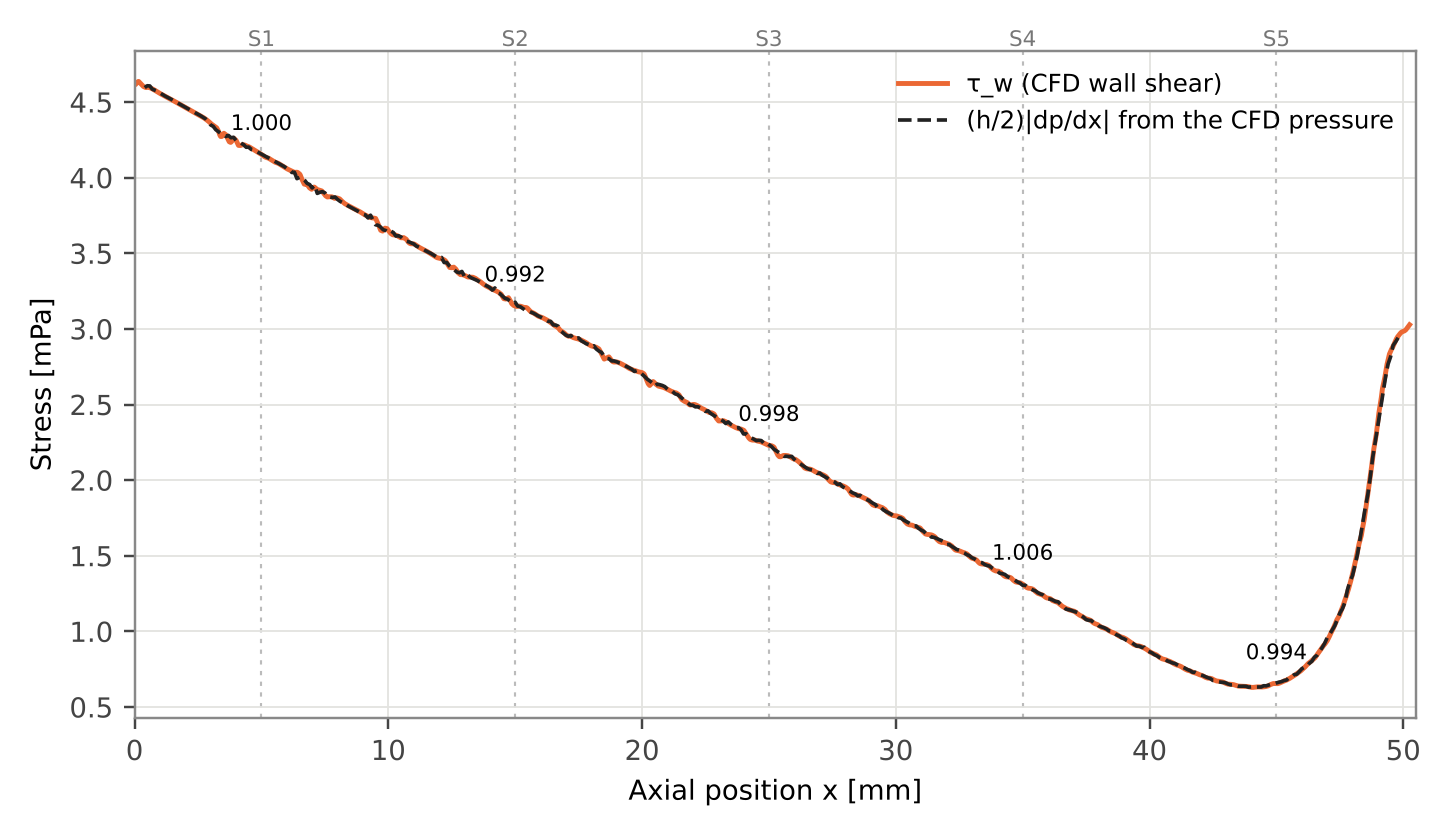
\includegraphics[width=\linewidth]{Fig38_pressure_gradient_vs_shear.png}
\caption{Momentum balance on the axis.}\label{fig:momentum}
\end{subfigure}\hfill
\begin{subfigure}[t]{0.49\linewidth}\centering
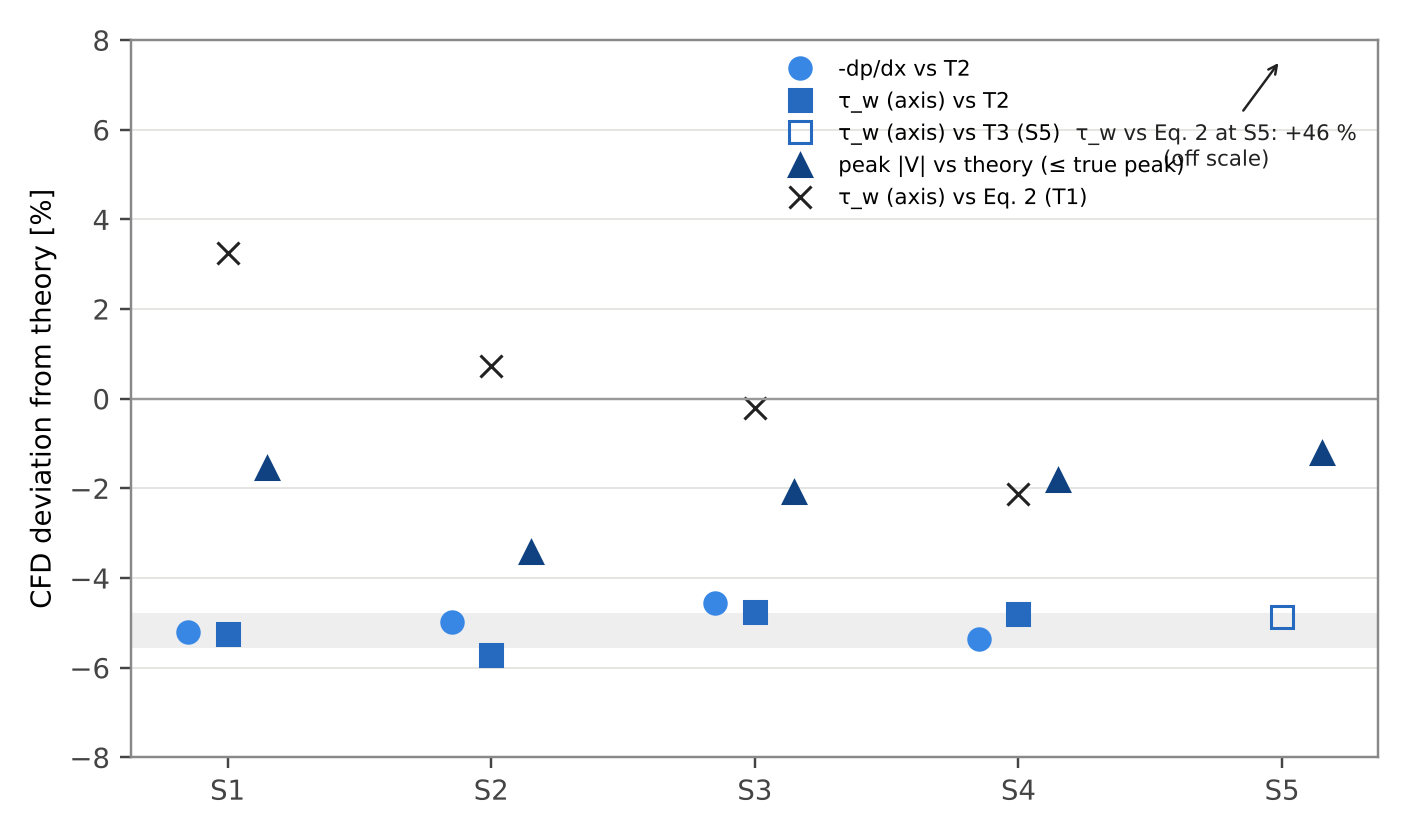
\includegraphics[width=\linewidth]{Fig37_validation_ratios_by_station.png}
\caption{Deviation from the best applicable theory.}\label{fig:val_ratios}
\end{subfigure}
\caption{(a) CFD wall shear against $(h/2)|\dd p/\dd x|$ from the CFD pressure; labels are the ratios \tagC. (b) Deviation of the CFD pressure gradient, wall shear and peak velocity from T2 (S1--S4) or T3 (S5); crosses mark Eq.~2. Pressure gradient and shear are uniformly about \SI{5}{\percent} low (grey band = mean $\pm$ s.d.\ over 2--\SI{40}{mm}); the peak velocity is within \SI{3.5}{\percent}. The S5 point against Eq.~2 (\SI{+46}{\percent}) is off-scale.}
\end{figure}

\section{Origin of the \texorpdfstring{\SI{-5}{\percent}}{-5 \%} offset}
\label{sec:val_offset}

Pressure gradient and wall shear are \SI{5.2(4)}{\percent} below the side-wall-corrected theory, uniformly in $x$ and identically at all three flow rates. Three causes are possible.
\begin{enumerate}
\item \textbf{Discretisation error across the gap (most likely).} About nine cell layers span $h$ everywhere, so an error caused by the wall-normal resolution has the same relative size at every station, as observed. Under-resolving the near-wall velocity gradient lowers the computed wall friction, and with it both the wall shear and the pressure gradient. These two stay mutually consistent (\cref{tab:momentum}). The decisive evidence is the velocity. The CFD peak velocity is \SIrange{1.6}{3.9}{\percent} \emph{higher} than $h^2|\dd p/\dd x|/8\mu$ (\cref{tab:velocity}, last column), which is the largest velocity that an exact parabolic profile with the CFD's own gradient can reach. Exceeding it is the signature of a discrete profile with too little wall friction.
\item \textbf{Flow deficit or incomplete convergence (less likely as the only cause).} A \SI{5}{\percent} lower flow rate would lower $p$, $\taw$ and $u$ by the same \SI{5}{\percent}. The peak velocity is, however, only 1.2--\SI{3.4}{\percent} below theory, and it is itself a lower bound because the sampled nodes are not exactly at mid-height. The missing mass-flux report means this cause cannot be fully excluded.
\item \textbf{A different channel height (unlikely).} A taller channel lowers $\Delta p\propto h^{-3}$, $\taw\propto h^{-2}$ and $u\propto h^{-1}$ by different amounts. No single $h$ can produce equal offsets in pressure gradient and shear, and the momentum balance gives $h=\SI{145(1)}{\micro\metre}$.
\end{enumerate}
The absolute CFD shear values should therefore be quoted as probably about \SI{5}{\percent} low until the mesh study of \cref{sec:num_gci} has been performed.

\section{Flow-rate scaling and regional behaviour}
\label{sec:val_scaling}

All interior quantities are proportional to $Q$ to within \SI{0.08}{\percent} (\cref{fig:scaling}a). The 0.22 and \SI{1}{\uLmin} cases agree to within \SI{0.001}{\percent}. At \SI{120}{\uLmin} ($\Rey_{D_h}=3.65$) the largest departures are \SI{+0.68}{\percent} for the shear peak at the inlet face and \SI{-0.8}{\percent} for the maximum velocity in the pathline images. Inertia therefore matters only at the inlet face of the lead-in, outside the measurement section, which confirms the Stokes-flow estimate of \cref{sec:dimensionless}.

\begin{figure}[htbp]
\centering
\begin{subfigure}[t]{0.49\linewidth}\centering
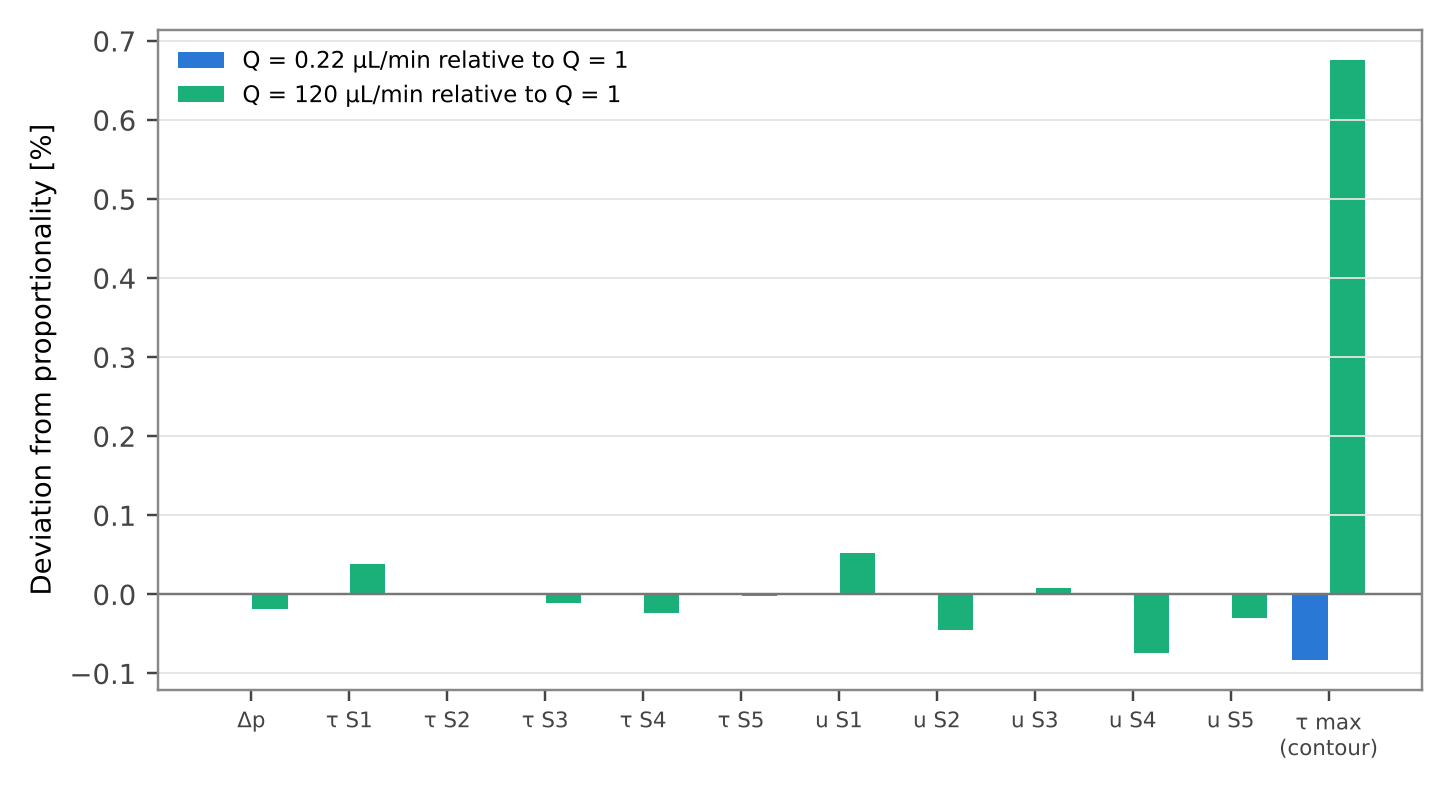
\includegraphics[width=\linewidth]{Fig40_flow_rate_scaling.png}
\caption{Departure from proportionality with $Q$.}
\end{subfigure}\hfill
\begin{subfigure}[t]{0.49\linewidth}\centering
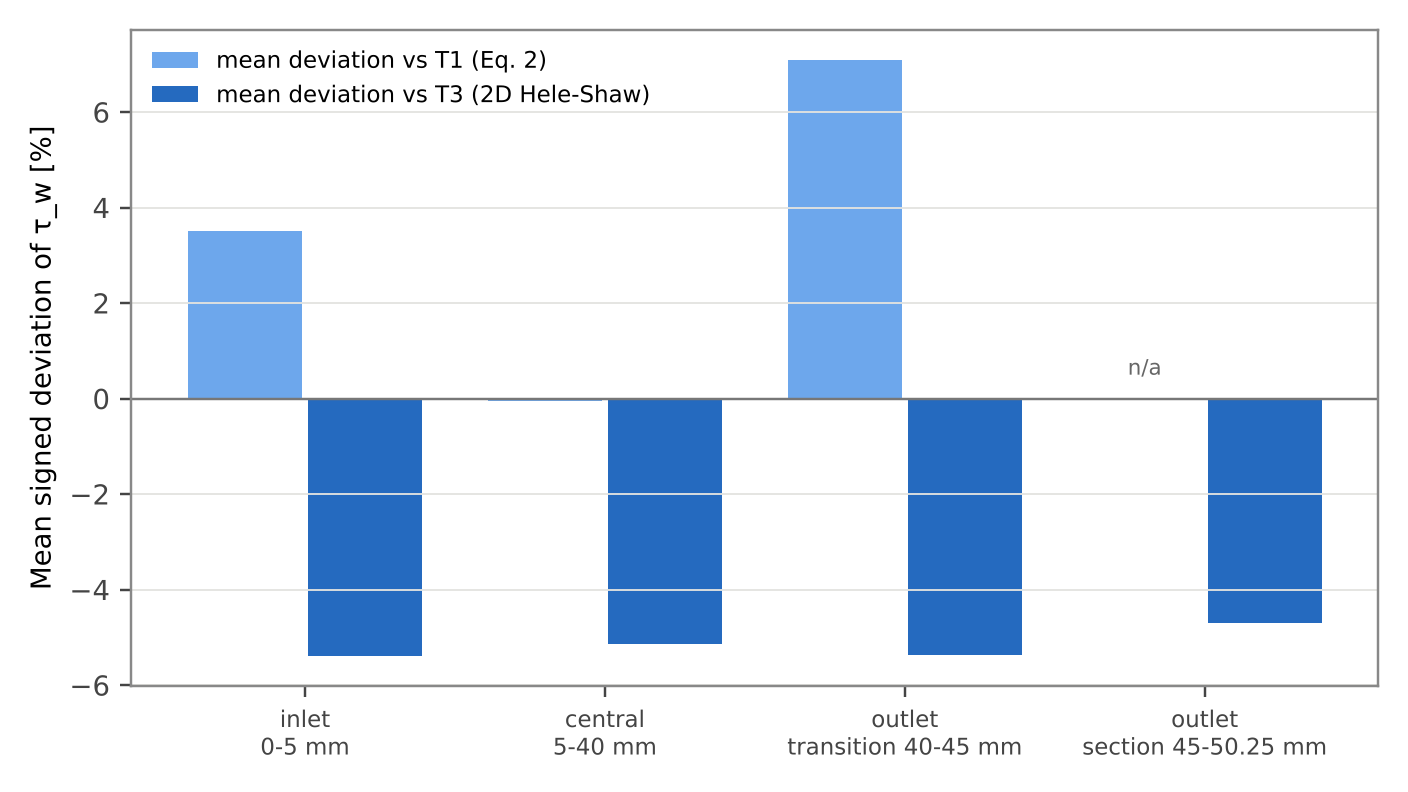
\includegraphics[width=\linewidth]{Fig41_regional_deviation.png}
\caption{Regional deviation of the axial shear.}
\end{subfigure}
\caption{(a) Percentage departure of each quantity from exact proportionality with $Q$, relative to \SI{1}{\uLmin} \tagC. (b) Mean signed deviation of the axial shear from Eq.~2, T2 and T3 in four regions (\SI{1}{\uLmin}). Eq.~2 is accurate on average in the central region but fails in the outlet transition; T3 removes the regional dependence and leaves the uniform \SI{-5}{\percent} offset.}
\label{fig:scaling}
\end{figure}

The regional analysis (\cref{fig:scaling}b) gives the following picture. In the inlet region (0--\SI{5}{mm}), the CFD exceeds Eq.~2 by \SI{3.5}{\percent} on average. In the central region (5--\SI{40}{mm}), the mean deviation is \SI{-0.05}{\percent}, although it ranges from \SI{+3.8}{\percent} to \SI{-3.1}{\percent} along $x$. In the outlet transition (40--\SI{45}{mm}), the mean deviation is \SI{+7.1}{\percent} and reaches \SI{+45}{\percent} at $x=\SI{45}{mm}$. Against T3 the mean deviation is between $-5.4$ and \SI{-4.7}{\percent} in every region.

\section{Physical interpretation of the flow field}
\label{sec:val_physics}

\paragraph{Velocity and flow distribution.} The flow is a Stokes flow in which each vertical column of fluid balances the local pressure gradient against the friction of the floor and the lid. The velocity profile across the gap is parabolic, and across the width it is flat except within about one gap height of the side walls. As the channel widens, the same flow is spread over a wider section, so the velocity falls as $1/w$, from \SI{0.17}{mm/s} at S1 to \SI{0.026}{mm/s} at S5 at \SI{1}{\uLmin}.

\paragraph{Pressure distribution and losses.} Since $\dd p/\dd x\propto1/w$, the pressure is lost mainly in the narrow upstream part: \SI{52}{\percent} of the T1 drop over the hyperbolic section occurs in its first \SI{15}{mm}, one third of its length. The resistance is linear, $R_{\mathrm{hyd}}=\SI{9.94e10}{Pa.s/m^3}$ from $x=0$ to the outlet, as expected for Stokes flow. The pressure drop of \SI{1.66}{Pa} at \SI{1}{\uLmin} is negligible for any syringe pump, but the corresponding velocities are very small. This becomes important for oxygen (\cref{ch:o2results}).

\paragraph{Wall shear.} The shear is set by the local pressure gradient, $\taw=(h/2)|\dd p/\dd x|$, and therefore falls as $1/w(x)$, i.e.\ linearly in $x$. Two effects modify this design behaviour. First, the side walls carry part of the drag, so for a given $Q$ a larger pressure gradient is needed, which raises the floor shear on the axis by $0.63\,h/w$. This is \SI{9}{\percent} at S1 and decreases downstream. Second, the converging outlet makes the flow two-dimensional within about \SI{3}{mm} of the corner: the iso-bars curve, the flow along the axis accelerates towards the outlet, and the shear passes through a minimum at \SI{44}{mm} and rises again. S5 lies exactly on this corner.

\paragraph{Development of the velocity profile.} The parabolic profile is established within $\sim\SI{0.09}{mm}$ of the inlet face and adapts instantly to the slow changes of width ($\Rey^*\ll1$). The flow is therefore locally fully developed everywhere in the hyperbolic section. There is no entrance effect at $x=0$ beyond a \SI{0.5}{\percent} local shear excess at $x\approx\SI{0.16}{mm}$, where the wall slope changes from zero (lead-in) to that of the hyperbola.

\paragraph{Local variations across the width.} The side-wall layer has a fixed thickness of about $0.9h$. Its share of the width shrinks downstream, so the region of uniform shear grows from \SI{70}{\percent} to \SI{91}{\percent} of the width between S1 and S4. This favours imaging in the downstream sections, up to the point where the outlet corner takes over.

\section{Validation summary}

\Cref{tab:validation_matrix} classifies each comparison.

\begin{table}[htbp]
\centering
\caption{Validation summary (\SI{1}{\uLmin}; other flow rates within \SI{0.1}{\percent}).}
\label{tab:validation_matrix}
\scriptsize
\begin{tabularx}{\linewidth}{@{}p{0.2\linewidth}p{0.22\linewidth}p{0.22\linewidth}X@{}}
\toprule
Quantity & Expectation & Observation & Classification and reason\\
\midrule
Published shear range \tagP & 0.01--0.001 and 0.0447--\SI{0.0059}{\dyncm} & 0.0102--0.0014 and 0.0464--\SI{0.0063}{\dyncm} & \textbf{Consistent} (semi-quantitative; published curves not tabulated)\\
Published imaging zone \tagP & $D_{\max}$ 0.34--\SI{3.84}{mm} & S3--S4 within \SI{2}{\percent}; S1--S2 +15 to \SI{+17}{\percent}; S5 differs & \textbf{Partly consistent}; criterion not stated in paper\\
Shape of $p(x)$ & T3 & $p/p(0)$ within \SI{0.08}{\percent} of T3 & \textbf{Quantitatively validated}\\
Magnitude of $\Delta p$ & T2/T3 & \SI{-4.9}{\percent} / \SI{-5.2}{\percent} & \textbf{Deviating} (uniform offset)\\
$\taw$ vs Eq.~2, S1--S4 & T1 & $+3.2$, $+0.7$, $-0.2$, \SI{-2.1}{\percent} & \textbf{Consistent}, but partly a cancellation of errors\\
Side-wall effect on $\taw$ & $1/f-1\approx0.63\,h/w$ & correct slope, offset \SI{-4.9}{\percent} & \textbf{Quantitatively validated} (slope)\\
Axial shape of $\taw$ & T3 ratios & within \SI{1}{\percent}, incl.\ S5 & \textbf{Quantitatively validated}\\
$\taw$ at S5 & T3: \SI{+54}{\percent} vs Eq.~2 & \SI{+46.5}{\percent} vs Eq.~2 & \textbf{Consistent}; Eq.~2 invalid at S5\\
Side-wall layer, uniform zone & \SI{0.129}{mm}; $d=w/2-0.129$ & 0.15--\SI{0.17}{mm}; $d$ 0.01--\SI{0.03}{mm} smaller & \textbf{Consistent} within node spacing\\
Transverse profile at S5 & T3 dome, $d=\SI{1.050}{mm}$ & dome, $d=\SI{1.024}{mm}$ & \textbf{Quantitatively validated}\\
Velocity across the width & flat core, side-wall layer & reproduced; peak 1.2--\SI{3.4}{\percent} low & \textbf{Consistent}\\
Velocity across the gap $u(z)$ & parabola & not exported & \textbf{Inconclusive} (no data)\\
Momentum balance & exact & within \SI{0.8}{\percent}; $h=\SI{145(1)}{\micro\metre}$ & \textbf{Quantitatively validated}\\
Peak velocity vs own gradient & $\le h^2|\dd p/\dd x|/8\mu$ & \SIrange{1.6}{3.9}{\percent} above & \textbf{Deviating}: under-resolved gap\\
Linearity in $Q$ & exact (Stokes) & within \SI{0.08}{\percent} & \textbf{Quantitatively validated}\\
Mesh independence & GCI from 3 meshes & one mesh only & \textbf{Inconclusive} (study pending)\\
\bottomrule
\end{tabularx}
\end{table}

\begin{keybox}[Answer to RQ1--RQ3]
The CFD reproduces every shape that the theory predicts: the axial distributions of pressure and shear (within \SI{1}{\percent}), the side-wall correction to Eq.~2 (with the correct slope), the side-wall layer, the dome-shaped profile at S5 and exact Stokes scaling. It also reproduces the published shear ranges and the published imaging zones at S3--S4. It does not yet reproduce the absolute magnitude: shear and pressure gradient are uniformly about \SI{5}{\percent} below the theory that includes side-wall drag, most probably because there are too few cells across the gap. Eq.~2 itself is accurate to $\pm\SI{4}{\percent}$ for $0\le x\lesssim\SI{40}{mm}$ only because the side-wall drag it omits and the CFD offset partly cancel. Eq.~2 fails at S5.
\end{keybox}
